\documentclass[12pt]{scrreprt}
\usepackage[utf8]{inputenc}
\usepackage[ngerman]{babel}
\usepackage[utf8]{inputenc}
\usepackage[T1]{fontenc}
\usepackage{hyperref}

%\hypersetup{colorlinks=true, citecolor=red}


\usepackage{natbib}
\usepackage[numbib]{tocbibind}
\usepackage{float}
\linespread{1.3}
\usepackage{natbib}
\usepackage{graphicx}
\usepackage{pdfpages}
\usepackage[euler]{textgreek}
\usepackage{adjustbox}
\usepackage[margin = 3cm]{geometry}


\usepackage{eso-pic} 
\usepackage{lipsum} 

\usepackage{tabularx} 
\usepackage{multirow}
\usepackage{amssymb}
\usepackage[flushleft]{threeparttable}
\usepackage{booktabs,caption}

\usepackage{amsmath}
\usepackage{bbm}
\usepackage{bbold}





\pagenumbering{roman}

\begin{document}
	
\pagestyle{myheadings}	
	
\begin{titlepage}
		\begin{center}
			\begin{minipage}{0.6\textwidth}%
				\begin{flushleft}
					Ludwig-Maximilians-Universität \\
					Institut für Statistik \\
					Wintersemester 2019/2020 \\
				\end{flushleft}
			\end{minipage}
			\begin{minipage}{0.35\textwidth}%
				\begin{flushright}
					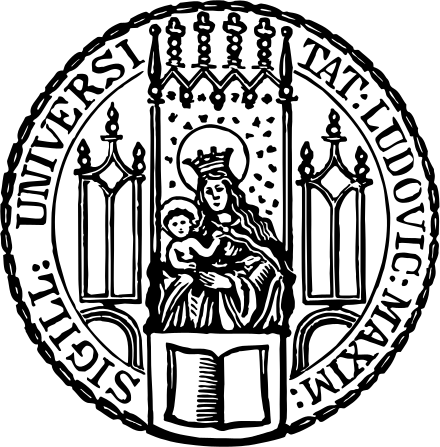
\includegraphics[scale = 0.2]{plots/lmu_logo}
				\end{flushright}
			\end{minipage}%
		\end{center}
		
		
		
		
		
		
		
		\vspace{4cm}
		
		{\centering
			{
				\Large\bfseries Abschlussbericht zum Projekt\\
				LVS-IR-Taubenstein\par}
			\vspace{9cm}
			\begin{flushleft}
				Projektpartner: Sascha Filimon, Roman Ossner\\ 
				Gruppenbetreuer: Dr. Andr\'{e} Klima\\ 
				Projektgruppe: Alexander Fogus, Lea Vanheyden, Zorana Spasojevi\'{c}
			\end{flushleft}
		}
\end{titlepage}
	
	
	
\newgeometry{top=1.25in,bottom=1.25in,right=1.25in,left=1.25in}	
\vspace{5cm}		
\thispagestyle{empty}
		
	%\newpage
	
	
\begingroup
	
	%\hypersetup{colorlinks=true, citecolor=black, linkcolor=black}
	
\tableofcontents	
\newpage	
\listoffigures	
\listoftables	
\setcounter{page}{1}
\thispagestyle{empty}		
\endgroup
	
\newpage	
\pagenumbering{arabic}

\chapter*{Abstract}
\setcounter{page}{1}
Im Rahmen dieser Arbeit und in Zusammenarbeit mit der Sektion München und Oberland des Deutschen Alpenvereins und des Departements für Geographie der Ludwig-Maximilians-Universität München wurden die Auswirkungen von Umwelteinflüssen auf die Mitnahme von Lawinenverschüttungssuchgeräte untersucht. \\
Ziel der vorliegenden Analyse ist die Untersuchung der Auswirkungen einzelner Parameter auf den Anteil von Personen, die ein solches Gerät bei sich tragen. \\
Diese Ergebnisse sollen helfen das Verhalten der Personen besser einschätzen und es in Folge auch besser steuern zu können. Beispiele der Kovariablen sind das Datum, die Uhrzeit, die Temperatur und die Lawinenwarnstufe. Als Datengrundlage dienen Messungen zweier Checkpoints im Gebiet Taubenstein, welche in der Wintersaison 2018/19 erhoben wurden. \\
Es wurden zwei Modelle, beides Generalisierte Additive Modelle mit der Binomial-Verteilung und der Logit-Link Funktion, geschätzt. Die beiden Modelle aggregieren die Daten auf unterschiedlichen Ebenen, so dass das eine Modell die Kovariable Uhrzeit au"ser Acht lässt. Aus beiden Modellen lassen sich schließlich die Zusammenhänge der Kovariablen mit dem Anteil der Personen mit LVS-Gerät ermitteln. Am Auffälligsten ist dabei eine generelle Abnahme des Anteils über die Saison. Ebenfalls zu beobachten sind bestimmte Uhrzeiten, an denen der Anteil höher ist und ein steigender zu erwartender Anteil mit der Lawinenwarnstufe. \\
Neben den Daten der Saison 18/19 wurden auch Daten zu zwei Tagen im Februar 2020 analysiert. Das Ziel war es hierbei mögliche Messfehler der Messgeräte quantifizieren zu können. Es wurde festgestellt, dass die Messgeräte ungefähr 22\% der vorbeilaufenden Personen nicht identifizieren. \\
Auf der Grundlage der Erkenntnis, dass Messfehler vorliegen wurde dann eine Sensitivitätsanalyse durchgeführt. Verschiedene Unterschätzungsszenarien wurden an den Daten simuliert, die Modelle darauf angewandt und dann miteinander verglichen. Die Szenarien sind: eine generelle Unterschätzung (dabei wird stufenweise von 10\% bis auf 70\% vorgegangen), eine Unterschätzung von Gruppen und eine Unterschätzung bei niedrigen Temperaturen. \\
Neben den Unterschätzungen wurde auch ein Überschätzungsszenario durchgeführt und nachts Messungen entfernt, da sie von Wildtieren stammen könnten. Alle Szenarien zeigen kaum Unterschiede in der Art des Effekts der Kovariablen. Einzig die Höhe des zu erwartenden Anteils nimmt ab oder zu.


\chapter{Einleitung}
Die Bayerischen Berge sind der Lebensraum zahlreicher Wildtiere. Jedoch nutzen auch Menschen die Alpen. Vor allem im Winter dringen Bergsportler in die Rückzuggebiete der Tiere ein und stören diese. \\
Der Deutsche Alpenverein versucht diese Konflikte zu entschärfen. Die Besucher werden vor Ort informiert und sollen durch Lenkungsmaßnahmen gesteuert werden. Dazu ist es nötig das Verhalten der Besucher zu verstehen. Dafür werden Signale von Lawinenverschüttungssuchgeräten ausgewertet und analysiert. Von Interesse ist deshalb auch ob, und unter welchen Umständen Wintersportler ein solches Gerät bei sich tragen. \\
Im Rahmen des statistischen Praktikums im Wintersemester 2019/20 und in Zusammenarbeit mit dem Deutschen Alpenverein Sektion München und Oberland und dem Department für Geografie der Ludwig-Maximilians-Universität München wurden in diesem Projekt die Auswirkungen verschiedener Umwelteinflüsse auf den Anteil der Personen die ein LVS-Gerät bei sich tragen untersucht. \\
Grundlage der Analyse sind dabei von zwei Checkpoints am Berg Taubenstein erhobene Messungen während der Wintersaison 2018/19. Neben den Checkpointmessungen liegen auch Daten zu Wetterbedingungen vor. Aus diesen Daten werden zwei Modelle geschätzt und analysiert. Dabei handelt es sich um generalisierte additive Modelle mit der Binomialverteilung und einer Logit-Link-Funktion. Die Validität der Modelle ist allerdings nur gegeben, wenn die für sie benutzten Daten keine strukturellen Fehler aufweisen. \\
Es wurde jedoch erkannt, dass die Messgeräte, welche die Daten über die Mitnahme der LVS-Geräte liefern fehlerhaft sind. Um das Ausmaß des Messfehlers feststellen zu können wurden im Februar 2020 manuelle Zählungen von Studierenden durchgeführt. Diese werden analysiert und auf Basis der Ergebnisse und Überlegungen der Projektpartner werden verschiedene Szenarien von fehlerhaften Messungen identifiziert. Diese werden an den Daten simuliert und die Modelle werden darauf angewandt. So möchte man untersuchen, welche Auswirkungen verschiedene Arten von Messfehlern auf die Ergebnisse des Modells haben. \\
Im Folgenden wird kurz auf den Hintergrund des Projekts genauer eingegangen. Danach werden die Daten beschrieben bevor zur Theorie hinter den Modellen übergegangen wird. Die praktischen Schwierigkeiten werden besprochen und die angewandten Modelle aufgezeigt. Im Anschluss werden die Ergebnisse beider Modelle besprochen und verglichen. Danach folgt die Messfehleranalyse. Zuerst werden die Zählungen der Studierenden deskriptiv betrachtet. Daraus werden dann vier Szenarien abgeleitet und für beide Modelle durchgeführt. Die Ergebnisse werden dann verglichen. Das Szenario der generellen Unterschätzung wird anschließend noch in 10\%-Schritten angewandt und verglichen. Abschlie"send wird ein Fazit gezogen.


\chapter{Hintergrund}

Für viele Besucher sind die Bayrischen Alpen ein beliebtes Gebiet, im Sommer sind Wanderer anzutreffen und im Winter vorrangig Skitouren- und Schneeschuhgeher. Jedoch stellt das Alpengebiet auch das Territorium von verschiedenen Tierarten dar. Es ist zu beobachten, dass es immer wieder zu räumlichen Konfliktsituation zwischen Menschen und Tieren kommt. Vor allem im Winter dringen die Sportler tief in die Rückzugsgebiete der Tiere ein und zwingen diese zur Flucht. \\
Um die räumlichen Konflikte zu entschärfen, werden die Besuchenden vor Ort informiert und durch Lenkungsmaßnahmen gesteuert. Mit dem Ziel einen nachhaltigen Tourismus gewährleisten zu können wurde ein Aktionstag seitens des Alpenvereins initiiert. Der Aktionstag ist ein Bestandteil der Kampagne „Natürlich auf Tour“ und dient der Sensibilisierung von Besuchern für einen verantwortungsvollen Umgang mit der Natur. 
(\cite{Alpenverein}) \\
Um das Besucherverhalten besser zu verstehen und beeinflussen zu können, werden die Signale der LVS-Geräts, das ein Skitourengeher in der Regel dicht am Körper trägt, ausgewertet und analysiert. \\
Ein LVS-Gerät ist ein Lawinenverschüttungssuchgerät und gehört zur Ausrüstung von Sportlern die in Schneegebieten unterwegs sind. Mit Hilfe eines LVS-Geräts können Personen, die von einer Lawine verschüttet worden sind, geortet werden. \\
Die Untersuchung über die Mitnahme von LVS-Geräten wurde anhand von Checkpoints gemessen. An den LVS-Checkpoints kann der Wintersportler sein Gerät auf dessen Funktionalität testen. Wenn eine Person ein eingeschaltetes LVS-Gerät bei sich trägt und an einem Checkpoint vorbei läuft, wird dies als ein LVS-Signal registriert und das Gerät leuchtet grün auf. Falls eine Person, die kein Gerät dabei hat, bzw. eins mit sich führt, dieses jedoch nicht eingeschaltet ist am Checkpoint vorbeiläuft, dann wird dies als eine Infrarot-Signal (abgekürzt: IR-Signal) identifiziert und das Messgerät leuchtet rot auf. \\
Die dabei anonym erhobenen Daten werden für die weitere Untersuchung betrachtet. \\
In unserem Projekt betrachten wir nicht das ganze Alpengebiet als Untersuchungsort, sondern beschränken uns auf den Spitzingsee. \\
\begin{figure}[H]
	\centering
	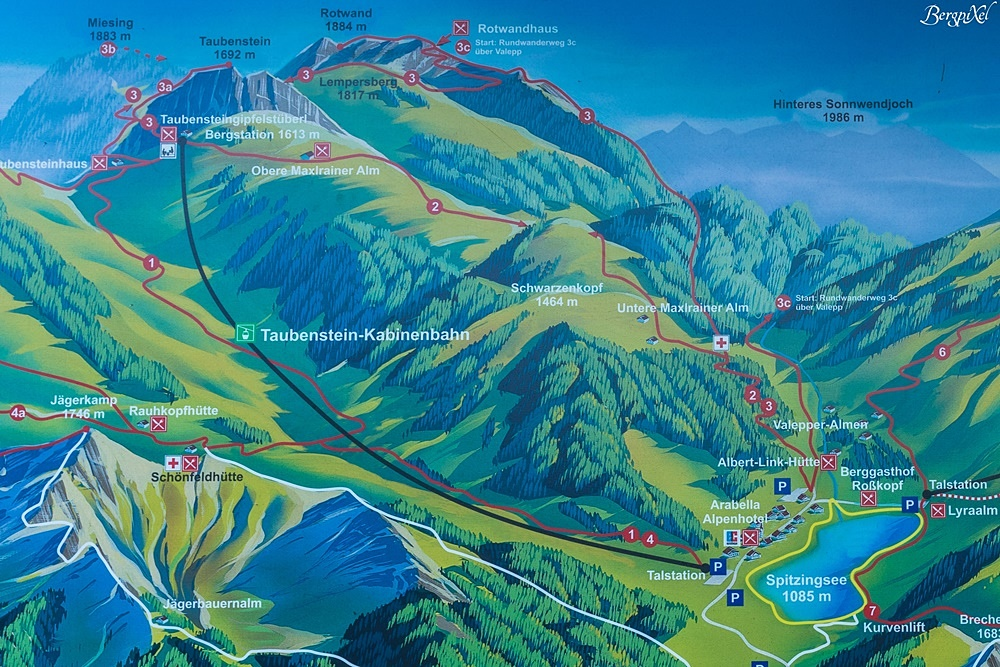
\includegraphics[width=\linewidth]{plots/spitzingsee}
	\caption{Untersuchungsraum: Spitzingsee mit dem Berg Taubenstein \\ (Bildquelle: Bergpixel.de)}
	\label{pic:spitzingsee}	
\end{figure}
%(Quelle: https://www.bergpixel.de/spitzingsee-rotwand-taubenstein-3/)
\noindent Der Spitzingsee ist ein beliebter Anlaufpunkt für Skitouren- und Schneeschuhgeher, aber auch das Revier von Wildtieren und daher als Untersuchungsraum für das Projekt geeignet.  Am Taubenstein-Parkplatz sind zur Hochsaison zwischen 500 bis 1000 Besucher anzutreffen, weshalb dieser Punkt für das Aufstellen von zwei Checkpoints genutzt wurde. %(Quelle: Panorama-6-2018-Skitouren-naturvertäglich-Bayern.pdf) \\
\begin{figure}[H]
	\centering
	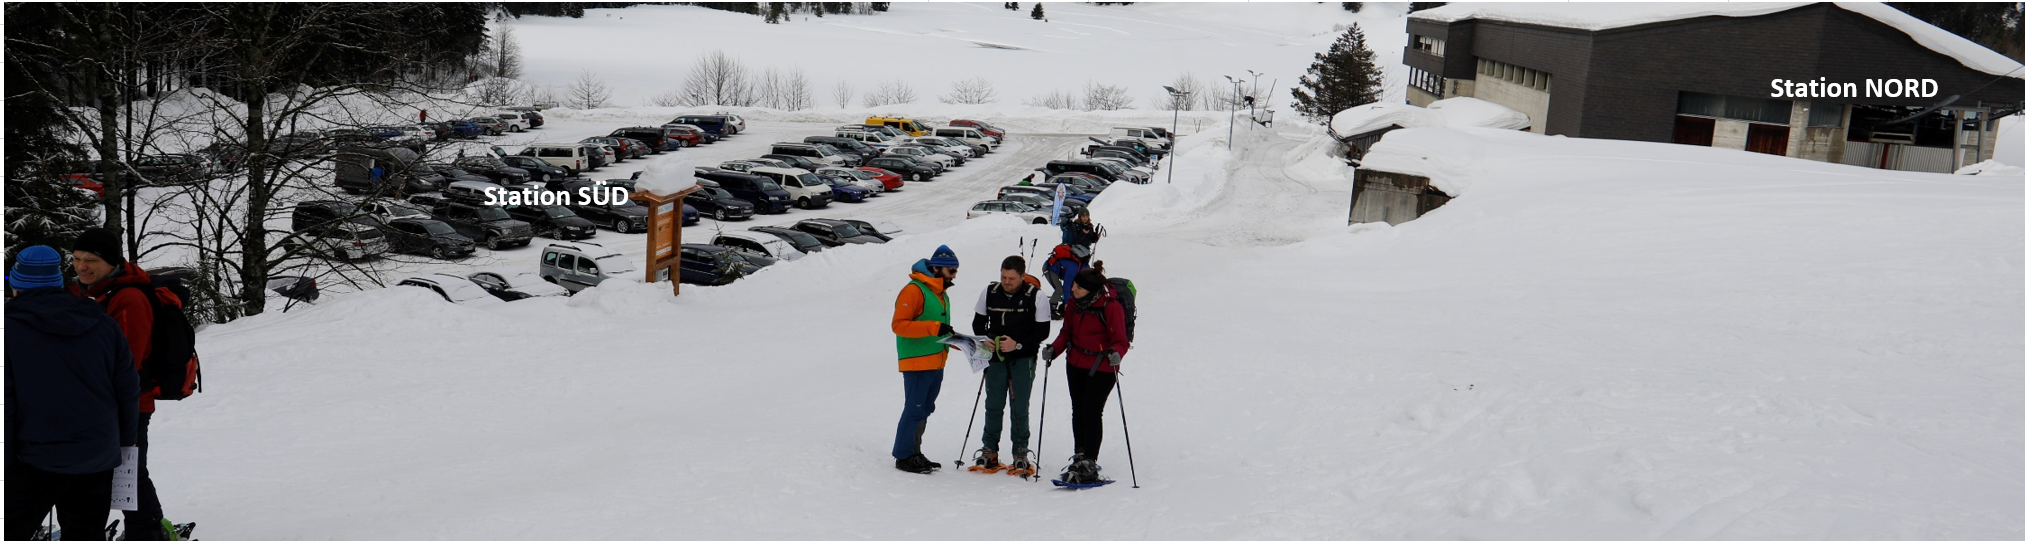
\includegraphics[width=\linewidth]{plots/checkpoint}
	\caption{LVS-Checkpoints an der Nord und Südseite des Taubenstein-Parkplatzes (Bildquelle: Roman Ossner DAV)}
	\label{pic:checkpoint}	
\end{figure}
\noindent Es gibt insgesamt zwei Checkpoints die einmal auf der Nord- und Südseite des Parkplatzes kurz vor Aufstieg des Bergs aufgestellt sind. \\
Im Fokus der Analyse steht der Zusammenhang zwischen dem Anteil der Besucher mit LVS-Gerät an allen Besuchern und verschiedenen Umweltfaktoren. Die von den Checkpoints generierten Daten werden im nächsten Kapitel näher beschrieben. 

\chapter{Datengrundlage}
In diesem Kapitel wird ein Überblick über die Datengrundlage des Projekts LVS-IR-Taubenstein gegeben. \\
Zuerst werden die im Zeitraum 2018/19 erhobenen Daten beschrieben. Da bekannt war, dass die Messgeräte fehlerhaft aufzeichnen, wurde im Februar 2020, seitens des Departments für Geographie eine manuelle Erhebung durchgeführt. Diese werden anschlie"send kurz beschrieben, im \autoref{chap:Messfehleranalyse} Messfehleranalyse wird genauer darauf eingegangen. \\
Die Messdaten wurden vom DAV München und Oberland und vom Department für Geographie der LMU zur Verfügung gestellt.

\section{Erhebungszeitraum 2018/2019}
In der Wintersaison 2018/2019 wurden die Daten von zwei Checkpoints an der Nord- und Südseite des Spitzingsee-Parkplatzes erfasst. Die Checkpoints registrieren dabei mithilfe von Infrarotsignalen, eine Person ohne LVS-Gerät bzw. mit ausgeschaltetem LVS-Gerät, sowie mittels eines LVS-Signals Personen mit eingeschaltetem LVS-Gerät. \\
Im Messzeitraum vom 21.12.2018 bis zum 13.04.2019 wurden insgesamt 37593 Messungen erfasst. Da die Messgeräte zeitweise aufgrund von starkem Schneefall bedeckt waren und nicht richtig messen konnten oder andersweitig nicht valide gemessen haben wurden die Daten für den Zeitraum vom 21.12.2018 bis zum 25.12.2018 und vom 07.01.2019 bis 15.01.2019 entfernt. \\
Damit bleiben 37216 Messungen übrig. Darunter wurden 28911 Personen ohne LVS-Gerät und 8305 Personen mit LVS-Gerät von den beiden Checkpoints registriert. \\
Die Messgeräte lösen bei jeder vorbeigehenden Person aus, wodurch auch Mehrfacherfassungen möglich sind. Das führt dazu, dass eine Person zum Beispiel beim Losgehen und Zurückkommen vom Checkpoint doppelt erfasst wird. \\
\subsection*{Zielvariable:}
\begin{itemize}
	\item Anteil der Personen mit LVS-Gerät
\end{itemize}
\subsection*{Kovariablen:}
\begin{itemize}
	\item Datum
	\item Wochentag
	\item Ferientag
	\item Schneehöhe (in cm)
	\item Temperatur (in ◦C)
	\item Lawinenwarnstufe
	\item Bewölkung
	\item Uhrzeit der Messung
	\item (Position)
\end{itemize}
Nachfolgend werden die zur Analyse des Modells erforderlichen Variablen vorgestellt.

\newpage
\subsubsection*{Anteil der Personen mit LVS-Gerät:}
Bei der Zielvariable handelt es sich um den Anteil der Personen mit bei geführtem LVS-Gerät an allen Personen die an den Checkpoints vorbeilaufen.
Kovariablen:
\subsubsection*{Datum:}
Es liegen wie oben erwähnt Daten vom 25.12.2018 bis zum 06.01.2019 und vom 16.01.2019 bis zum 13.04.2019 vor. \\
Das Balkendiagramm (\ref{pic:date_lvs}) zeigt die absolute Häufigkeit der Messungen nach Datum und Art der Messung. Hier zu erkennen sind die fehlenden Messungen im Zeitraum vom 07.01.2019 bis zum 15.01.2019.
\begin{figure}[H]
	\centering
	\includegraphics[width=\linewidth]{plots/date_lvs}
	\caption{Balkendiagramm der absoluten Häufigkeit der Messungen mit und ohne LVS-Gerät nach Datum}
	\label{pic:date_lvs}	
\end{figure}

\newpage
\noindent Da der Anteil der Personen mit LVS-Gerät von Interesse ist, ist dieser in (\ref{pic:date_ratio}) über die Saison hinweg zu sehen. Auch hier sind die fehlenden Tage ersichtlich. Zu erkennen ist ein sinkender Anteil der Personen mit LVS-Gerät über den Verlauf der Saison. Jedoch sind starke Schwankungen zu beobachten.
\begin{figure}[H]
	\centering
	\includegraphics[width=\linewidth]{plots/date_ratio}
	\caption{Liniendiagramm für den Anteil der Personen mit LVS-Gerät nach Datum}
	\label{pic:date_ratio}	
\end{figure}

\newpage
\subsubsection*{Wochentag:}
Anhand der Variable Datum konnte der Wochentag mit den Ausprägungen von Montag bis Sonntag festgelegt werden. \\
Die absoluten Häufigkeiten der Checkpoint-Messungen nach Wochentag sind in Abbildung (\ref{pic:day_plot}) zu sehen. Es ist zu beobachten, dass am Wochenende die Anzahl der Personen insgesamt (mit und ohne LVS-Gerät) im Vergleich zu den restlichen Tagen am höchsten ist. 
\begin{figure}[H]
	\centering
	\includegraphics[width=\linewidth]{plots/day_plot}
	\caption{Gestapeltes Balkendiagramm der absoluten Häufigkeit der Personen mit und ohne LVS-Gerät nach Wochentag}
	\label{pic:day_plot}	
\end{figure}

\newpage
\subsubsection*{Ferientag:}
Bei jeder Messung ist au"serdem bekannt, ob es sich bei dem Datum um einen Ferientag gehandelt hat. Unter den Begriff Ferientag fallen sowohl Feiertage als auch Schulferientage in Bayern. Insgesamt gibt es 22 Ferientage. \\
Die absoluten Häufigkeiten der Personen mit und ohne LVS-Gerät nach Ferientag sind in Abbildung (\ref{pic:holiday_plot}) zu sehen.
\begin{figure}[H]
	\centering
	\includegraphics[width=\linewidth]{plots/holiday_plot}
	\caption{Gestapeltes Balkendiagramm der absoluten Häufigkeiten der Personen mit und ohne LVS-Gerät für den Fall, dass es sich um einen Ferientag handelt und für den Fall, dass es sich nicht um einen Ferientag handelt}
	\label{pic:holiday_plot}	
\end{figure}

\newpage
\subsubsection{Schneehöhe:}
Zu jeder Messung liegt die tägliche Schneehöhe in cm vor. Der Verlauf der Schneehöhe über die Wintersaison wird in Abbildung (\ref{pic:date_snowhight}) dargestellt. \\
Dabei ist zu erkennen, dass die Schneehöhe von Mitte Dezember bis Mitte Januar tendenziell steigt. \\
Von Mitte Januar bis Mitte Februar ist der höchste Schnee zu beobachten, wobei Schwankungen sichtbar sind. Ab Mitte Februar ist eine absteigende Tendenz der Schneehöhe zu sehen. Der höchste Wert für die Schneehöhe beträgt 212 cm und der niedrigste Wert 16 cm. 
\begin{figure}[H]
	\centering
	\includegraphics[width=\linewidth]{plots/date_snowhight}
	\caption{Liniendiagramm der Schneehöhe in cm nach Datum (ausgegraute Werte an Tagen die aus dem Datensatz entfernt wurden)}
	\label{pic:date_snowhight}	
\end{figure}
\noindent Die Kovariable Schneehöhe wurde aufgrund des Concurvity-Problems transformiert, worauf in \autoref{chap:Concurvity} näher eingegangen wird.
  
\newpage
\subsubsection*{Temperatur:}
Die Variable Temperatur wurde um 12 Uhr mittags des jeweiligen Tages in Grad Celsius erhoben. Tendenziell ist in Abbildung (\ref{pic:date_temperature}) ein steigender Temperaturverlauf mit starken Schwankungen von Ende Dezember bis Mitte April zu beobachten. Die niedrigste gemessene Temperatur beträgt -7,9 Grad Celsius und die Höchste 9,7 Grad Celsius. 
\begin{figure}[H]
	\centering
	\includegraphics[width=\linewidth]{plots/date_temperature}
	\caption{Liniendiagramm der Temperatur in $^\circ$C um 12 Uhr mittags nach Datum (ausgegraute Werte an Tagen die aus dem Datensatz entfernt wurden; horizontale, gestrichelte Linie kennzeichnet 0 Grad Celsius)}
	\label{pic:date_temperature}	
\end{figure}

\newpage
\subsubsection*{Lawinenwarnstufe:}
Die Variable Lawinenwarnstufe besteht aus dem Durchschnitt zweier anderer Variablen, nämlich der Lawinenwarnstufe am Fu"s und an der Spitze des Berges, welche täglich erhoben wurden. Es gibt Warnstufen von eins bis fünf, wobei fünf die grö"sste Gefahr bedeutet. \\
In Abbildung (\ref{pic:boxplot_avalanche_report}) wird anhand eines Boxplots die Verteilung der Variable ersichtlich. Zu beobachten ist, dass der Median bei Warnstufe zwei liegt. Ebenfalls erkennbar ist, dass die Lawinenwarnstufe fünf in unserem Datensatz nicht vorkommt. Die höchste vorkommende Lawinenwarnstufe ist vier und die Niedrigste, die auch das 25\%-Quantil darstellt, ist eins. 
\begin{figure}[H]
	\centering
	\includegraphics[width=\linewidth]{plots/boxplot_avalanche_report}
	\caption{Boxplot der täglichen Durchschnittslawinenwarnstufe}
	\label{pic:boxplot_avalanche_report}	
\end{figure}

\newpage
\subsubsection*{Bewölkung:}
Die Bewölkung wird als Anteil von 100\% angegeben. Eine 100-prozentige Bewölkung bedeutet ein komplett bedeckter Himmel und 0-prozentige Bewölkung ein wolkenfreier Himmel. Im Gegensatz zu den anderen bisher genannten Kovariablen liegt der Anteil der Bewölkung nicht täglich, sondern stündlich vor. \\
Es wurde neben dem stündlichen Wert auch der tägliche Durchschnittswert errechnet. Dieser ist in Abbildung (\ref{pic:date_cloud_cover}) zu sehen, wobei eine starke Schwankung erkennbar ist.
\begin{figure}[H]
	\centering
	\includegraphics[width=\linewidth]{plots/date_cloud_cover}
	\caption{Liniendiagramm der täglichen Durchschnittsbewölkung in Prozent nach Datum (ausgegraute Werte an Tagen die aus dem Datensatz entfernt wurden)}
	\label{pic:date_cloud_cover}	
\end{figure}

\newpage
\subsubsection*{Uhrzeit der Messung:}
Zu jeder Messung registriert das Messgerät neben dem Datum auch die Uhrzeit. Die absolute Häufigkeit der Personen mit und ohne LVS-Gerät nach der Uhrzeit wird in Abbildung (\ref{pic:time_lvs}) dargestellt. \\
Im Zeitraum zwischen 10 Uhr und 20 Uhr ist die Anzahl der Personen insgesamt (mit und ohne LVS-Gerät) am höchsten. \\
Wie auch schon am Anfang des Kapitels erwähnt, kann dieselbe Person mehrfach registriert werden. So werden Besucher, die erst nach Mitternacht des nächsten Tages von ihrer Tour zurückkehren erneut registriert. Bei ihrer Entscheidung, ob sie ein LVS-Gerät mitnehmen haben sie sich jedoch wahrscheinlich an den Umwelt-Bedingungen des Aufbruchtages orientiert. \\
Deshalb wurde, in Absprache mit den Projektpartnern, beschlossen den Tag von 4 Uhr morgens bis 4 Uhr morgens des eigentlich nächsten Tages laufen zu lassen. Einer Messung von 0 Uhr bis 4 Uhr werden daher die Kovariablen des Vortags zugeordnet. 
\begin{figure}[H]
	\centering
	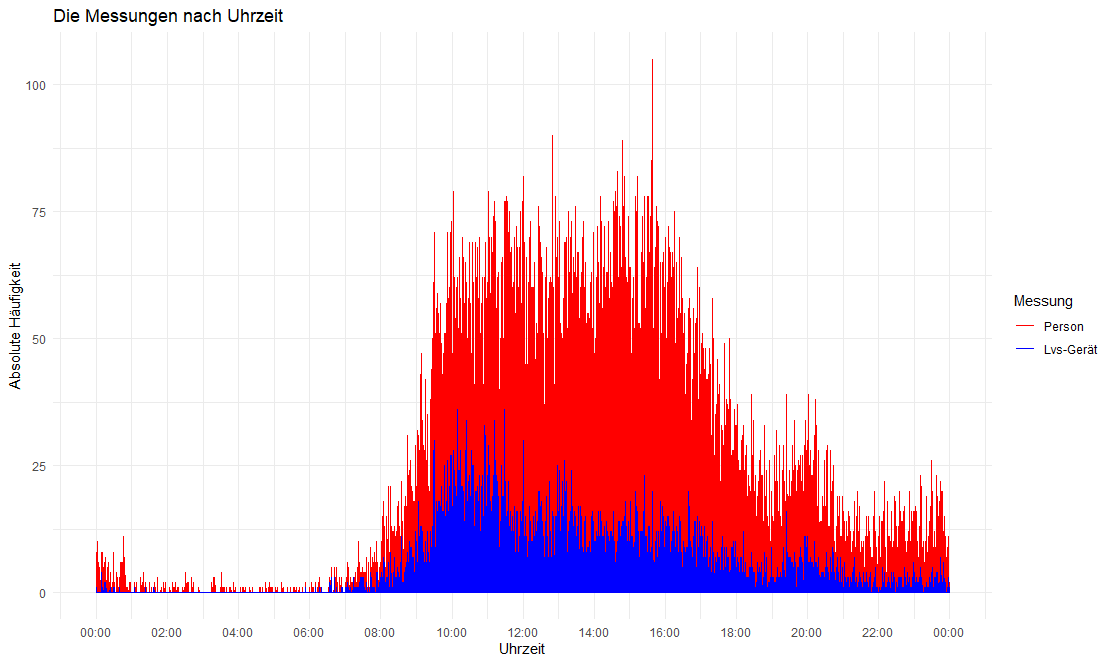
\includegraphics[width=\linewidth]{plots/time_lvs}
	\caption{Balkendiagramm der absoluten Häufigkeit der Personen mit und ohne LVS-Gerät nach Uhrzeit der Messung (vertikale Linie kennzeichnet den neuen Tagesbeginn)}
	\label{pic:time_lvs}	
\end{figure}

\newpage
\subsubsection*{Position:}
Neben den bisher erwähnten Variablen ist bei jeder Messung auch der Ort des Messgerätes bekannt, also ob die Person vom Nord- oder Süd-Checkpoint registriert wurde. \\
Die absoluten Häufigkeiten über die Wintersaison hinweg sind in Abbildung (\ref{pic:date_position}) zu sehen. Es ist zu erkennen, dass deutlich mehr Personen am Süd-Checkpoint gemessen wurden. Für die folgenden Modelle wurden jedoch die Messungen der beiden Checkpoints zusammengezählt und die Position au"ser Acht gelassen.
\begin{figure}[H]
	\centering
	\includegraphics[width=\linewidth]{plots/date_position}
	\caption{Balkendiagramm der absoluten Häufigkeit der Messungen nach Datum, aufgeteilt nach Position des Checkpoints (Nord und Süd)}
	\label{pic:date_position}	
\end{figure}

\noindent Die Messungen für die Variablen Schneehöhe, Temperatur und Lawinenwarnstufe wurden nicht von den Checkpoints am Spitzingsee gemessen, sondern von dem Gewässerkundlichen Dienst Bayern erhoben. Die Messungen der Variable Bewölkung stammen von Meteoblue %(ref: https://www.meteoblue.com/de/wetter/woche/taubenstein_deutschland_2823864).

\section{Erhebungszeitraum 2020}
Da erkannt wurde, dass die Messgeräte teilweise fehlerhaft messen, wurden manuelle Zählungen der Studierenden des Departments für Geografie durchgeführt. \\
Der Erhebungszeitraum beschränkt sich auf den 27.02.2020 und 28.02.2020. An diesen Tagen wurden nur Zählungen am Checkpoint-Nord durchgeführt (da der Checkpoint-Süd ausgefallen ist). \\
Diese sollen dabei helfen mögliche Strukturen des Messfehlers zu erkennen. Dabei haben die Studierenden beobachtet, ob eine vorbeilaufende Person vom Checkpoint registriert wird. Jede vorbeigehende Person wurde notiert und ebenso wurde vermerkt, ob diese vom Checkpoint erkannt wurde. Dabei wurde nicht zwischen Person mit und ohne LVS-Gerät unterschieden.\\ Die Studierenden haben außerdem angegeben, ob es sich bei der Person um einen Skitourengänger oder einen anderen Kontakt handelt. \\
Neben den Daten der Studierenden liegen auch die vom Checkpoint erhobenen Daten vor. Insgesamt wurden von den Studierenden 208 Personen gezählt und von den Checkpoints 170 Messungen erfasst. Die aus diesen Daten gewonnen Erkenntnisse und deren Auswirkungen werden in \autoref{chap:Messfehleranalyse} beschrieben. 

\chapter{Methodik}
In diesem Kapitel wird als erstes die Theorie hinter den Modellen erklärt. Danach wird auf die aufgetretenen Schwierigkeiten und die angewandten Lösungen eingegangen. Im letzten Teil werden die Ergebnisse der Modelle besprochen.

\section{Theorie}
In folgendem Kapitel soll die Theorie hinter den Modellen erklärt werden. Für das bessere Verständnis wird der Theorie-Teil von einem einfachen Modell bis hin zu dem von uns verwendeten Modell aufgebaut. \\
Die mathematischen Formeln und Konzepte aus diesem Kapitel basieren, wenn nicht anders vermerkt, aus dem Buch \glqq{Regression-Modelle, Methoden und Anwendungen}\grqq ~von Ludwig Fahrmeir et al..

\subsection{Lineares Regressionsmodell}
Das einfachste Regressionsmodell ist das lineare Regressionsmodell. Hierbei wird der Erwartungswert einer Zielvariable durch die Linearkombination von Einflussgrö"sen, auch Kovariablen genannt, beschrieben. Das lineare Regressionsmodell nimmt dabei folgende Form an:
\begin{align}
y_{i}= \beta_{0}+\beta_{1}x_{i1}+...+\beta_{k}x_{ik}+\epsilon_{i}
\end{align}
Die Zielgrö"se, $y_{i}$, muss stetig und approximativ normalverteilt sein. Die Kovariablen werden durch $x_{i1},...,x_{ik}$ gekennzeichnet und $\epsilon_{i}$ stellt den Störterm dar. In Anwendungen bei denen es sich nicht um eine normalverteilte Zielvariable handelt ist das lineare Regressionsmodell unzureichend. (\cite{fahrmeir2007regression} S.20 ff.) \\
Dieses Problem löst das generalisierte lineare Regressionsmodell, auf welches im nächsten Abschnitt eingegangen wird. 

\subsection{Generalisiertes lineares Regressionsmodell}
Das generalisierte lineare Regressionsmodell eignet sich für die Modellierung von Zielvariablen die nicht normalverteilt sind. Die abhängige Variable kann eine Verteilung aus der Exponentialfamilie (z.B. Binomial, Poisson, Multinomial, Normal,...)annehmen. Durch eine Link-Funktion wird sie dann in eine normalverteilte Variable transformiert. \\
Bei den später verwendeten Modellen lässt sich die Zielvariable wie folgt beschreiben: \\
\begin{align}
%\vspace{0.1cm}
y_{i}=\begin{cases}
1 & \text{,wenn Person mit LVS-Gerät gemessen wird } \\
0 & \text{,wenn Person ohne LVS-Gerät gemessen wird.} \\
\end{cases}
\end{align}
Die beobachtete Zielvariable ist Binomial-verteilt mit $y_{i}|x_{i}\sim B(1,\pi_{i})$. \\

Bei der generalisierten Regression mit binärer Zielvariable, wie in diesem Fall, wird der Effekt der Kovariablen durch die (bedingte) Wahrscheinlichkeit $\pi_{i}$ beschrieben.
\begin{align}
\pi_{i}=P(y_{i}=1|x_{i1},...,x_{ik})=E(y_{i}|x_{i1},...,x_{ik})
\end{align}
Für den Erwartungswert der Zielvariable gilt:
\begin{align}
E(y_{i})=\pi_{i}=\frac{exp(\eta_{i})}{1+exp(\eta_{i})}=h(\eta_{i}).
\end{align}
Der Erwartungswert der Zielvariable wird mit dem linearen Prädiktor $\eta_{i}$ mittels der Responsefunktion $\pi_{i}=h(\eta_{i})$ verknüpft. Die Logit-Linkfunktion $g$ ist die Umkehrung der Responsefunktion, daher gilt:
\begin{align}
g(\pi_{i})=\log(\frac{\pi_{i}}{1-\pi_{i}}).
\end{align}
Die hier verwendeten Modelle machen Gebrauch von dem Logit-Link. \\
Das generalisierte lineare Regressionsmodell beschreibt lineare Einflüsse der Kovariablen auf die Zielvariable. In praktischen Anwendungen ist dies oft unzureichend, da neben den linearen Einflüssen auch nicht-lineare, flexible Einflüsse von Kovariablen auf die abhängige Variable wirken können. (\cite{fahrmeir2007regression} S.189 ff.) Daher wird im nächsten Kapitel die additive Regression näher erläutert.

\subsection{Additives Regressionsmodell}
Das additive Modell stellt ein semi-parametrisches Regressionsmodell dar. Neben linearen Einflüssen können auch nicht-lineare flexible Einflüsse von Kovariablen auf die abhängige Variable modelliert werden. \\
Das Standardmodell der additiven Regression hat die Form:
\begin{align}
y_{i}=\underbrace{\beta_{0}+\beta_{1}x_{i1}+...+\beta_{k}x_{ik}}_{\text{parametrische Effekte}}+ \underbrace{f_{1}(z_{i1})+...+f_{q}(z_{iq})}_{\text{nichtparametrische Effekte}}+\epsilon_{i}
\end{align}
Der parametrische Teil des Standardmodells hat die gleiche Form, wie schon im linearen Modell aufgezeigt. Die Funktionen $f_{1}(z_{1}),...,f_{q}(z_{q})$ sind sogenannte Glättungen und schätzen die nichtparametrischen Effekte. (\cite{fahrmeir2007regression} S.44 ff.) \\
Auf die Theorie hinter den glatten Funktionen $f$ wird im nächsten Kapitel eingegangen.

\subsection{Splines}
Die Glättungsfunktion $f$ wird durch sogenannte Splines modelliert. Splines stellen bestimmte Funktionen dar, die stückweise aus Polynomen eines bestimmten Grades zusammengesetzt werden. Es gibt verschiedene Arten von Splines. (\cite{fahrmeir2007regression} S. 291 ff.) \\
In den Modellen wurden die Penalisierten Splines, die Zyklische Splines und die Thin-Plate Splines verwendet. Im Folgenden werden diese erläutert, wobei zum einfacheren Verständnis zuvor noch Polynom- und Basis-Splines erklärt werden.

\subsubsection{Polynom-Splines}
Eine Möglichkeit, die Funktion $f$ abzubilden, sind Splines, die über Polynome modelliert werden und Polynom-Splines, oder auch Regressions-Splines, genannt werden. Das polynomiale Modell hat die Form: 
\begin{align}
f(z)=\gamma_{0}+\gamma_{1}z+...+\gamma_{l}z^l,
\end{align}
wobei das Polynom vom Grad $l$ durch den Einfluss von $z$ auf $y$ modelliert wird und $\gamma_{j}$ die Regressionskoeffizienten darstellen. Um eine flexible Schätzfunktion gewährleisten zu können, wird der Definitionsbereich von $z$ in Intervalle geteilt und Polynome werden für das jeweilige Intervall geschätzt. Die Zerlegung von $z$ erfolgt stückweise auf Basis von sogenannten Knotenmengen $k_{1}$ bis $k_{m}$.  Ein Problem, welches dabei entstehen könnte ist, dass an den Intervallgrenzen keine $glatte$ Funktion entstehen. Der Graph einer $glatten$ Funktion hat an den Intervallgrenzen keine \glqq{Ecken\grqq}. Deshalb muss für die \glqq{mathematische}\grqq ~Glattheit die zusätzliche Bedingung, dass die Funktion $f(z)$ an den Intervallgrenzen $(l-1)$-mal stetig differenzierbar ist, eingeführt werden. Der Grad des Splines und die Anzahl der Knoten können im hohen Ma"se die Funktion beeinflussen, je höher die Anzahl an Knoten ist, desto $rauer$ ist die Funktion $f(z)$. Um Polynom-Splines in der Praxis anwenden zu können, bedarf es einer Darstellung der Menge der Polynom-Splines. Eine mögliche Darstellung eines Polynom-Splines stellt die B-Spline-Basisfunktion dar. (\cite{fahrmeir2007regression} S.293 ff.)

\subsubsection{Basis Splines}
Der B-Spline dient als Basisfunktion für Polynom-Splines. Jedoch wird sich auch der Penalisierungs-Spline, welcher im folgenden Abschnitt vorgestellt wird, die B-Spline-Basisfunktion zu Nutzen machen. Das Ziel bei der Konstruktion der B-Spline-Basisfunktion ist es die Polynomstücke des gewünschten Grades an den Knoten ausreichend $glatt$ zusammenzusetzen. Die Basisfunktion besteht dabei aus $(l+1)$ Polynomstücken vom Grad $l$, welche stetig an den Knoten zusammengesetzt werden. Die Funktion $f(z)$ lässt sich durch die Linearkombination der Basisfunktionen:
\begin{align}
f(z)=\sum_{j=1}^d\gamma_{j}B_{j}(z)
\end{align}
darstellen. Die Koeffizienten  $\gamma_{j}$ werden mit Hilfe der KQ-Methode geschätzt und dienen zur Skalierung der Basisfunktionen. Die Anzahl der erforderlichen Basisfunktionen $d = m+l-1$, setzt sich aus der Zahl der Knoten $m$ und den Polynomstücken des gewünschten Grades $l$, welche $(l-1)$-mal stetig differenzierbar an den Knoten aneinandergefügt werden, zusammen.  \\
Für B-Splines vom Grad 0 folgt:
\begin{align}
B_{j}^0(z)= \mathbb{1}_{[k_{j},k_{j+1}]}(z)= 
\begin{cases}
1 & k_{j} \leq z<k_{j+1};\enspace mit\enspace j=1,...,d-1; \\
0 & \text{sonst.} \\
\end{cases}
\end{align}
Für B-Splines höheren Grades gilt:
\begin{align}
B_{j}^l(z)= \frac{z-k_{j}}{k_{j+l}-k_{j}}B_{j}^{l-1}(z)+
\frac{k_{j+l+1}-z}{k_{j+l+1}-k_j+1}B_{j+1}^{l-1}(z).
\end{align}
(\cite{fahrmeir2007regression} S.303 ff.) \\
Die Abbildung \ref{pic:b_spline} visualisiert die Schätzung eines B-Splines anhand eines fiktiven Datenbeispiels schematisch. Abbildung (a) demonstriert eine B-Spline Basis vom dritten Grad. In Abbildung (b) wird die Basisfunktion mit dem Kleinste-Quadrate-Schätzer $\hat\gamma_{j}$ skaliert. Die Abbildung (c), zeigt die erhaltene Schätzung, wenn die skalierten Basisfunktionen addiert werden.
\begin{figure}[H]
	\centering
	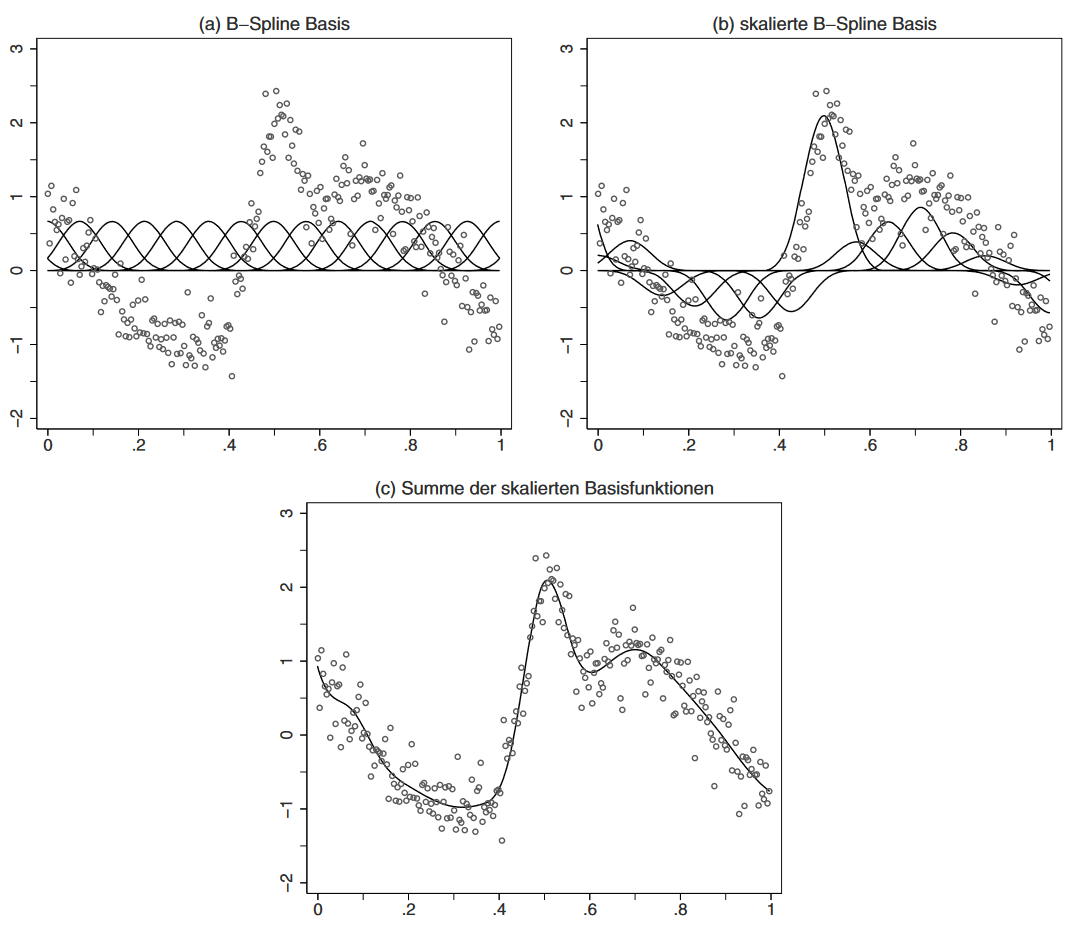
\includegraphics[width=\linewidth]{plots/b_spline.png}
	\caption{Schematische Darstellung der Schätzung eines nichtparametrischen Effekts mit B-Splines (\cite{fahrmeir2007regression} S.307)}
	\label{pic:b_spline}
\end{figure}

\noindent Das nächste Kapitel behandelt P-Splines, welche auf B-Splines basieren und durch einen Strafterm erweitert worden sind. Diese werden  bei den später erklärten Modellen verwendet.

\subsubsection{Penalisierte Splines basierend auf B-Splines}
Bereits im vorherigen Abschnitt wurde klar, dass die Knotenmenge einen wichtigen Faktor darstellt. Die Glattheit und Flexibilität der Schätzfunktion $f(z)$ hängt stark von der Anzahl der Knoten ab. Eine zu hohe Anzahl von Knoten führt zu sogenanntem \glqq Overfitting\grqq, das hei"st die Funktion ähnelt zu sehr den Daten und ist sehr wacklig. Die Idee der P-Splines ist es die Funktion $f(z)$ auf Basis einer B-Spline Funktion mit einer gro"sen Zahl an Knoten zu approximieren um so die Flexibilität der Schätzfunktion sicherzustellen und andererseits zu hohe Variabilität durch einen Strafterm zu sanktionieren. Die Knoten Für die Penalisierten Splines wurden in den angewandten Modellen nach Perzentilen gesetzt. Das dient dazu, die Knoten dahin zu setzen wo vielen Beobachtungen sind, um an diesen Stellen mehr Flexibilität zu erreichen. Der Penalisierte-Spline, gekürzt P-Spline, kombiniert somit eine B-Spline-Basis mit einem Strafterm. Der Strafterm für B-Splines wird durch die quadrierte zweite Ableitung der Schätzfunktion $f(z)$ modelliert. Die zweite Ableitung stellt ein Ma"s für die Krümmung der Funktion dar und ist daher in der Lage die Glattheit einer Funktion einzuschätzen.
Der Strafterm: 
\begin{align}
\lambda\int(f''(z))^2dz.
\end{align}
In der Anwendung wird für die Approximation der zweiten Ableitungen, die zweite Differenz des Parameters $\gamma_{j}$ verwendet. Wenn der Glättungsparameter $\lambda$ gegen unendlich konvergiert, erhält man eine nahezu lineare Schätzfunktion $f(z)$. Im Fall von $\lambda \to 0$ konvergiert auch der Strafterm gegen $0$ und die P-Splines verhalten sich wie unpenalisierte B-Splines. Der Glättungsparameter $\lambda$ wird im Modell durch REML (Restriktierte Maximum-Likelihood) geschätzt. (\cite{fahrmeir2007regression} S.309 f.)

\subsubsection{Zyklische P-Splines}
Eine Glättungsfunktion hei"st zyklisch, wenn die Funktion dieselben Werte und ersten Ableitungen an ihrer oberen und unteren Grenze aufweist. Beispielsweise kann man die Funktion für die Variable Wochentag mit Hilfe des zyklischen P-Splines modellieren. Das Ziel dabei ist es z.B den Sonntag mit dem darauffolgenden Montag zu verknüpfen. Dadurch wird sichergestellt, dass die Werte am Ende einer Woche zusammenhängend zu den Werten am Anfang der darauffolgenden Woche sind. 
Die Schätzfunktion eines zyklischen P-Splines hat die Form:
\begin{align}
f(z)=\sum_{j=1}^{k-1}B_{j}(z)\beta_{j}.
\end{align}
Der Koeffizient $\beta_{j}$ wird durch den transponierten Vektor $\beta^T=(\beta_{1},...,\beta_{k-1})$ dargestellt, wobei $\beta_{j}=\beta_{k}$ gilt.
Der Penalisierungsansatz für zyklische P-Splines ist simultan zu der Penalisierung von P-Splines basierend auf B-Splines. (\cite{wood2017generalized} S.202 ff.)

\subsubsection{Thin-Plate Splines}
Bisher wurden Funktionen mit nur einer einzigen Kovariable geschätzt. Die Thin-Plate Splines ermöglichen die Schätzung einer Funktion mit mehreren Kovariablen. Bei dem hier angewandeten Modell handelt es sich um eine Funktion mit zwei Variablen, nämlich dem Datum und der Uhrzeit. Die beiden Variablen wurden in einer Funktion geschätzt, da sie miteinander interagieren. Der Vorteil von Thin-Plate Splines ist, dass nun eine Auswahl von Knotenpositionen oder Basisfunktionen nicht notwendig ist, da sich diese durch die mathematische Darstellung des Glättungsparameters ergibt. Die Glattheit, wenn $z$ zweidimensional ist, wird durch die Minimierung der Funktion von $f$ erzielt, die die folgende Form hat:
\begin{align}
||y-f||^2+\underbrace{\lambda}_{\substack{\text{Glättungs-} \\ \text{parameter}}} \underbrace{J_{md}(f)}_{\substack{\text{Straf-} \\ \text{term}}}.
\end{align}
Dabei stellt $y$ den Vektor von $y_{i}$ und $f=[(f(z_{1}),...,f(z_{n}))]^T$ dar. Die Funktion $f$ wird durch einen Glättungsparameter, multipliziert mit einem Strafterm für raue bzw. wackelige Funktionen ergänzt. (\cite{wood2017generalized} S.215 ff.)

\subsection{Generalisiertes additives Modell}
Das generalisierte additive Modell verbindet das additive Regressionsmodell mit einem generalisierten Modell.
Es eignet sich um nicht-lineare Effekte von metrischen Kovariablen auf eine nicht unbedingt normalverteilte Zielvariable zu beschreiben. Wie schon im additiven Modell erläutert, setzt sich der additive Prädiktor $(\eta_{i})$ aus einem parametrischen- und einem nichtparametrischen Teil zusammen.
\begin{align}
\eta_{i}=\underbrace{\beta_{0}+\beta_{1}x_{i1}+...+\beta_{k}x_{ik}}_{\text{parametrische Effekte}}+ \underbrace{f_{1}(z_{i1})+...+f_{q}(z_{iq})}_{\text{nichtparametrische Effekte}}+\epsilon_{i}
\end{align}
(\cite{fahrmeir2007regression} S.47 f.) \\
Bei den beiden angewandten Modelle handelt es sich um generalisierte additive Modelle mit einer Logit-Link-Funktion. Die glatten Funktionen werden mithilfe von P-Splines, zyklischen P-Splines und Thin-Plate-Splines geschätzt. Bevor im Kapitel (...)die konkreten Modelle vorgestellt werden, geht es im nächsten Abschnitt um aufgetretene Schwierigkeiten.

\section{Praktische Herausforderungen}
In diesem Teil der Arbeit wird ein Überblick über die Praktische Herausforderungen im Modell gegeben. Es wird als erstes das Concurvity-Problem erläutert, dann die Überdispersion und im letzten Abschnitt die Autokorrelation.

\subsection{Concurvity}
\label{chap:Concurvity}
Die Kollinearität beschreibt einen linearen Zusammenhang zwischen den Kovariablen. Die Concurvity kann als Erweiterung der Kollinearität angesehen werden und charakterisiert die nicht-lineare Zusammenhänge von Kovariablen. Ein hohes Ma"s an Concurvity weist daher auf einen starken Zusammenhang zwischen zwei oder mehreren Kovariablen hin. Durch das Auftreten der Concurvity kommt es zu einer Art Varianz-Inflation der geschätzten Regressionskoeffizienten. Das hei"st die Koeffizienten in dem generalisierten additiven Modell werden instabil. (\cite{amodio2014concurvity} S.88 f.) \\
Bei der Untersuchung der Kovariablen auf Concurvity zeigt sich einige leicht erhöhte Werte. Deshalb wird die Variable Schneehöhe zu Schneedifferenz transformiert. Die Schneedifferenz des jeweiligen Tages berechnet sich durch Subtraktion der Schneehöhe des vorherigen Tages von der Schneehöhe des jeweiligen Tages. Durch die Transformation der Kovariable Schneehöhe zu Schneedifferenz ist das Ma"s an Concurvity gesunken. In Abbildung (\ref{pic:date_snowdiff}) ist die neue Variable Schneedifferenz nach Datum zu sehen.

\begin{figure}[H]
	\centering
	\includegraphics[width=\linewidth]{plots/date_snowdiff}
	\caption{Liniendiagramm der Schneedifferenz zum Vortag in cm nach Datum (ausgegraute Werte an Tagen die aus dem Datensatz entfernt wurden)}
	\label{pic:date_snowdiff}	
\end{figure}

\subsection{Überdispersion}
Bei den bisher vorgestellten Modellen ist man von Individualdaten ausgegangen. Jeder Beobachtung wird genau ein Individuum aus der Stichprobe zugeordnet.
Bei den angewandten Datensätzen im Modell handelt es sich nicht um Individualdaten, sondern um gruppierte Daten. Die Individualdaten werden nach identischen Zeilen in der Datenmatrix gruppiert. (\cite{fahrmeir2007regression} S.195 f.) \\ 
In der Arbeit werden zwei Modelle angewendet, das Tagesmodell und das Zeitmodell. \\
Im Tagesmodell werden die Daten nach dem Tag bzw. Datum gruppiert, wodurch Datenmatrix insgesamt $n = 101$ Zeilen aufweist. Die Kovariable Uhrzeit wird dabei nicht beachtet. Da jedoch auch die Uhrzeit von Interesse für die Datenanalyse ist, wird ein zweites Modell, nämlich das Zeitmodell, aufgestellt. Im Zeitmodell werden die Individualdaten nach der Minute gruppiert und $n = 19334$ Beobachtungseinheiten erzeugt. Das Gruppieren von Individualdaten führt dazu, dass Anteile für Personen mit LVS-Gerät für das jeweilige Datum bzw. das Datum und die Uhrzeit berechnet werden. \\
Durch das Gruppieren nach Datum oder Minute kann es zur Überdispersion kommen. Das hei"st die Daten weisen eine grö"sere Streuung bzw. Varianz auf, als durch das Modell zu erwarten ist. Das Problem der Überdispersion wird durch das Einsetzen eines Dispersionsparameters in die Varianzformel gelöst.
\begin{align}
Var(y_{i}|\textbf{x}_{i})=\underbrace{\phi}_\text{Dispersionsparameter} \underbrace{\pi_{i}(1-\pi_{i})}_\text{Varianz}.
\end{align}
Der Dispersionsparameter wird errechnet durch:
\begin{align}
\phi=\frac{\text{Devianz}}{\text{Freiheitsgrade der Residuen}}.
\end{align} 
({(\cite{fahrmeir2007regression} S.195 f.)})

\subsection{Autokorrelation}
Die Autokorrelation beschreibt die Korrelation einer Funktion mit sich selbst zu einem früheren Zeitpunkt. In Zeitreihen entsteht das Problem der Autokorrelation häufig, da die Annahme der unkorrelierten Störgrö"sen verletzt ist. Man unterscheidet dabei zwischen der empirischen Autokorrelation (ACF) und der partiellen Autokorrelation (PACF).\\
Die empirische Autokorrelation wird berechnet durch:
\begin{align}
\widehat{\text{ACF}}(j)=\frac{\widehat{\text{Cov}}(\epsilon_{i},\epsilon_{i-j})}{\widehat{\text{Var}}(\epsilon_{i})} \quad \text{mit} \quad \widehat{\text{Cov}}(\epsilon,\epsilon_{i-j})=\frac{1}{n}\sum_{i=j+1}^{n}\hat{\epsilon}_{i}\hat{\epsilon}_{i-j}.
\end{align}
Dabei sind $\epsilon_{i}$ die Residuen und $\epsilon_{i-j}$ die um $j$ verzögerten Residuen. Das ACF gibt die Korrelation zwischen den Störungen $\epsilon_{i}$ und den um $j$ Perioden verzögerten Störtermen an. Das PACF hingegen berechnet die Korrelation zwischen $\epsilon_{i}$ und $\epsilon_{i-j}$ ohne den Einfluss der dazwischen liegenden Störungen zu beachten. Dabei ist:
\begin{align}
\epsilon_{i}=\alpha_{1}\epsilon_{i-1}+...+\alpha_{j}\epsilon_{i-j}
+v_{i},
\end{align}
wobei $\alpha_{j}$ der Regressionskoeffizient des Modells ist. Die partielle Autokorrelation PACF wird durch:
\begin{align}
\widehat{\text{PACF}}(j)=\hat{\alpha}_{j}
\end{align}
bestimmt. (\cite{fahrmeir2007regression} S.137 ff.)\\
Beide Modelle wurden auf Autokorrelation geprüft. Um das Problem der Autokorrelation genauer zu analysieren können die empirische Autokorrelation und partielle Autokorrelation anhand von sogenannten Korrelogrammen, wie in den Abbildungen (\ref{pic:ACF}) und (\ref{pic:PACF}), grafisch dargestellt werden. Die  Korrelogramme zeigen niedrige empirische- und partielle Autokorrelation bei beiden Modellen, wodurch keine weiteren Ma"snahmen zur Behebung der Autokorrelation erforderlich sind.
\begin{figure}[H]
	\centering
	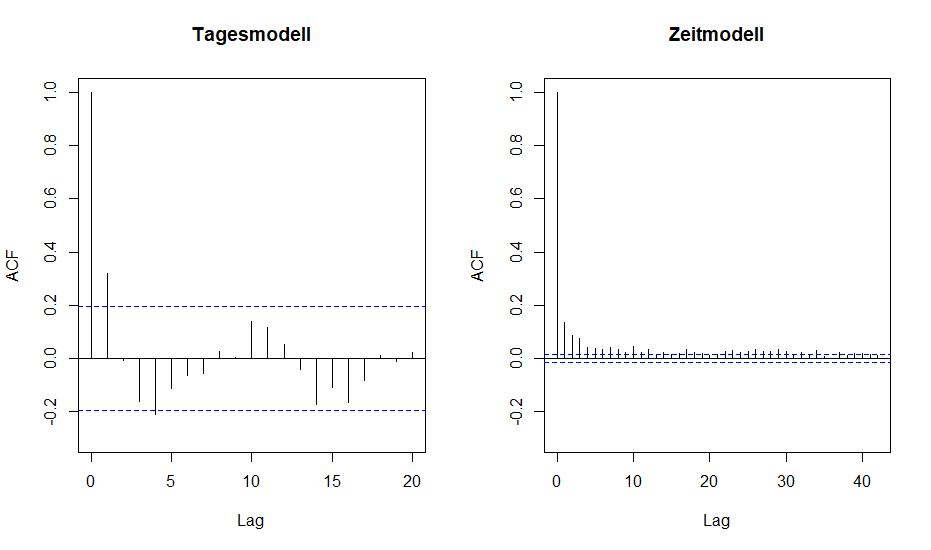
\includegraphics[width=\linewidth]{plots/ACF}
	\caption{Korrelogramm der Autokorrelation nach Verzögerung (Lag) für das Tages- und Zeitmodell}
	\label{pic:ACF}	
\end{figure}

\begin{figure}[H]
	\centering
	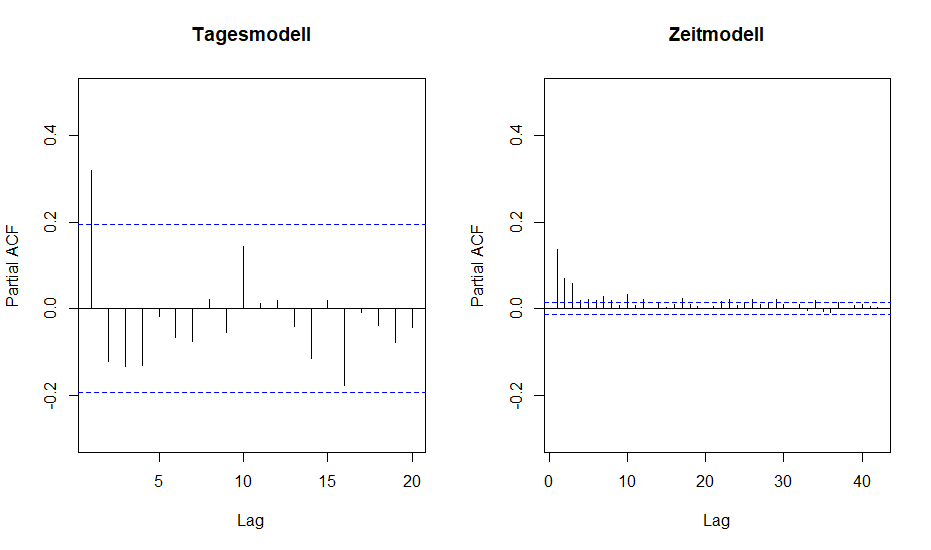
\includegraphics[width=\linewidth]{plots/PACF}
	\caption{Korrelogramm der partiellen Autokorrelation nach Verzögerung (Lag) für das Tages- und Zeitmodell}
	\label{pic:PACF}	
\end{figure}


\chapter{Angewandte Modelle}
Nach der Erläuterung des theoretischen Hintergrunds folgen nun die beiden bereits angesprochenen Modelle. Zuerst wird der zuvor allgemein erklärte additive Prädiktor für die beiden angewandten Modelle definiert. Danach werden die Ergebnisse der Modelle vorgestellt.

\section{Tagesmodell}
Das Tagesmodell ist ein generalisiertes additives Modell, bei dem die Messungen nach Datum gruppiert sind. Der additive Prädiktor sieht damit wie folgt aus:
\begin{align}
\begin{split}
\eta_{i}= ~ &\beta_{0}+\beta_{1}(\text{Ferientag}_{i})+ \\
&f_{1}(\text{Datum}_{i})+f_{2}(\text{Lawinenwarnstufe}_{i})+ \\
&f_{3}(\text{Wochentag}_{i})+ f_{4}(\text{Temperatur}_{i})+ \\ &f_{5}(\text{durchschnittliche Tages-Bewölkung}_{i})+ \\
&f_{6}(\text{Schneedifferenz}_{i}).
\end{split}
\end{align}

\section{Zeitmodell}
Das zweite Modell, das Zeitmodell, stellt ebenfalls ein generalisiertes additives Modell dar. Welches allerdings um die Variable Uhrzeit erweitert wurde und nach Minute gruppiert ist. Damit ergibt sich folgender additiver Prädiktor:
\begin{align}
\begin{split}
\eta_{i}= ~ &\beta_{0}+\beta_{1}(\text{Ferientag}_{i})+ \\
&f_{1,2}(\text{Uhrzeit}_{i},\text{Datum}_{i})+f_{3}(\text{Lawinenwarnstufe}_{i})+ \\
&f_{4}(\text{Wochentag}_{i})+f_{5}(\text{Temperatur}_{i})+ \\
&f_{6}(\text{stündliche Bewölkung}_{i})+ \\
&f_{7}(\text{Schneedifferenz}_{i}).
\end{split}
\end{align}
Bei der Funktion $f_{1,2}$ handelt es sich um einen sogenannten Interaktionseffekt. Das ist notwendig, wenn eine nicht-lineare Interaktion zwischen zwei oder mehreren Variablen besteht. Hier interagieren die Uhrzeit und das Datum miteinander.

\section{Ergebnisse}
Es werden die Ergebnisse des Tages- und des Zeitmodells vorgestellt und die beiden Modelle miteinander verglichen.
\subsection{Ergebnisse des Tagesmodells}
Das Modell umfasst n = 101 Tage an den Messungen vorliegen. 
Der Intercept ist der zu erwartende Anteil von Personen mit LVS-Gerät an einem Tag, der kein Ferientag ist und bei dem alle anderen Kovariablen durchschnittlich sind. Der Intercept des Tagesmodells beträgt 21,67\%. An einem Ferientag mit ansonsten durchschnittlichen Variablen wird ein Anteil von Personen mit LVS-Gerät in Höhe von 19,71\% erwartet. \\
\begin{figure}[H]
	\centering
	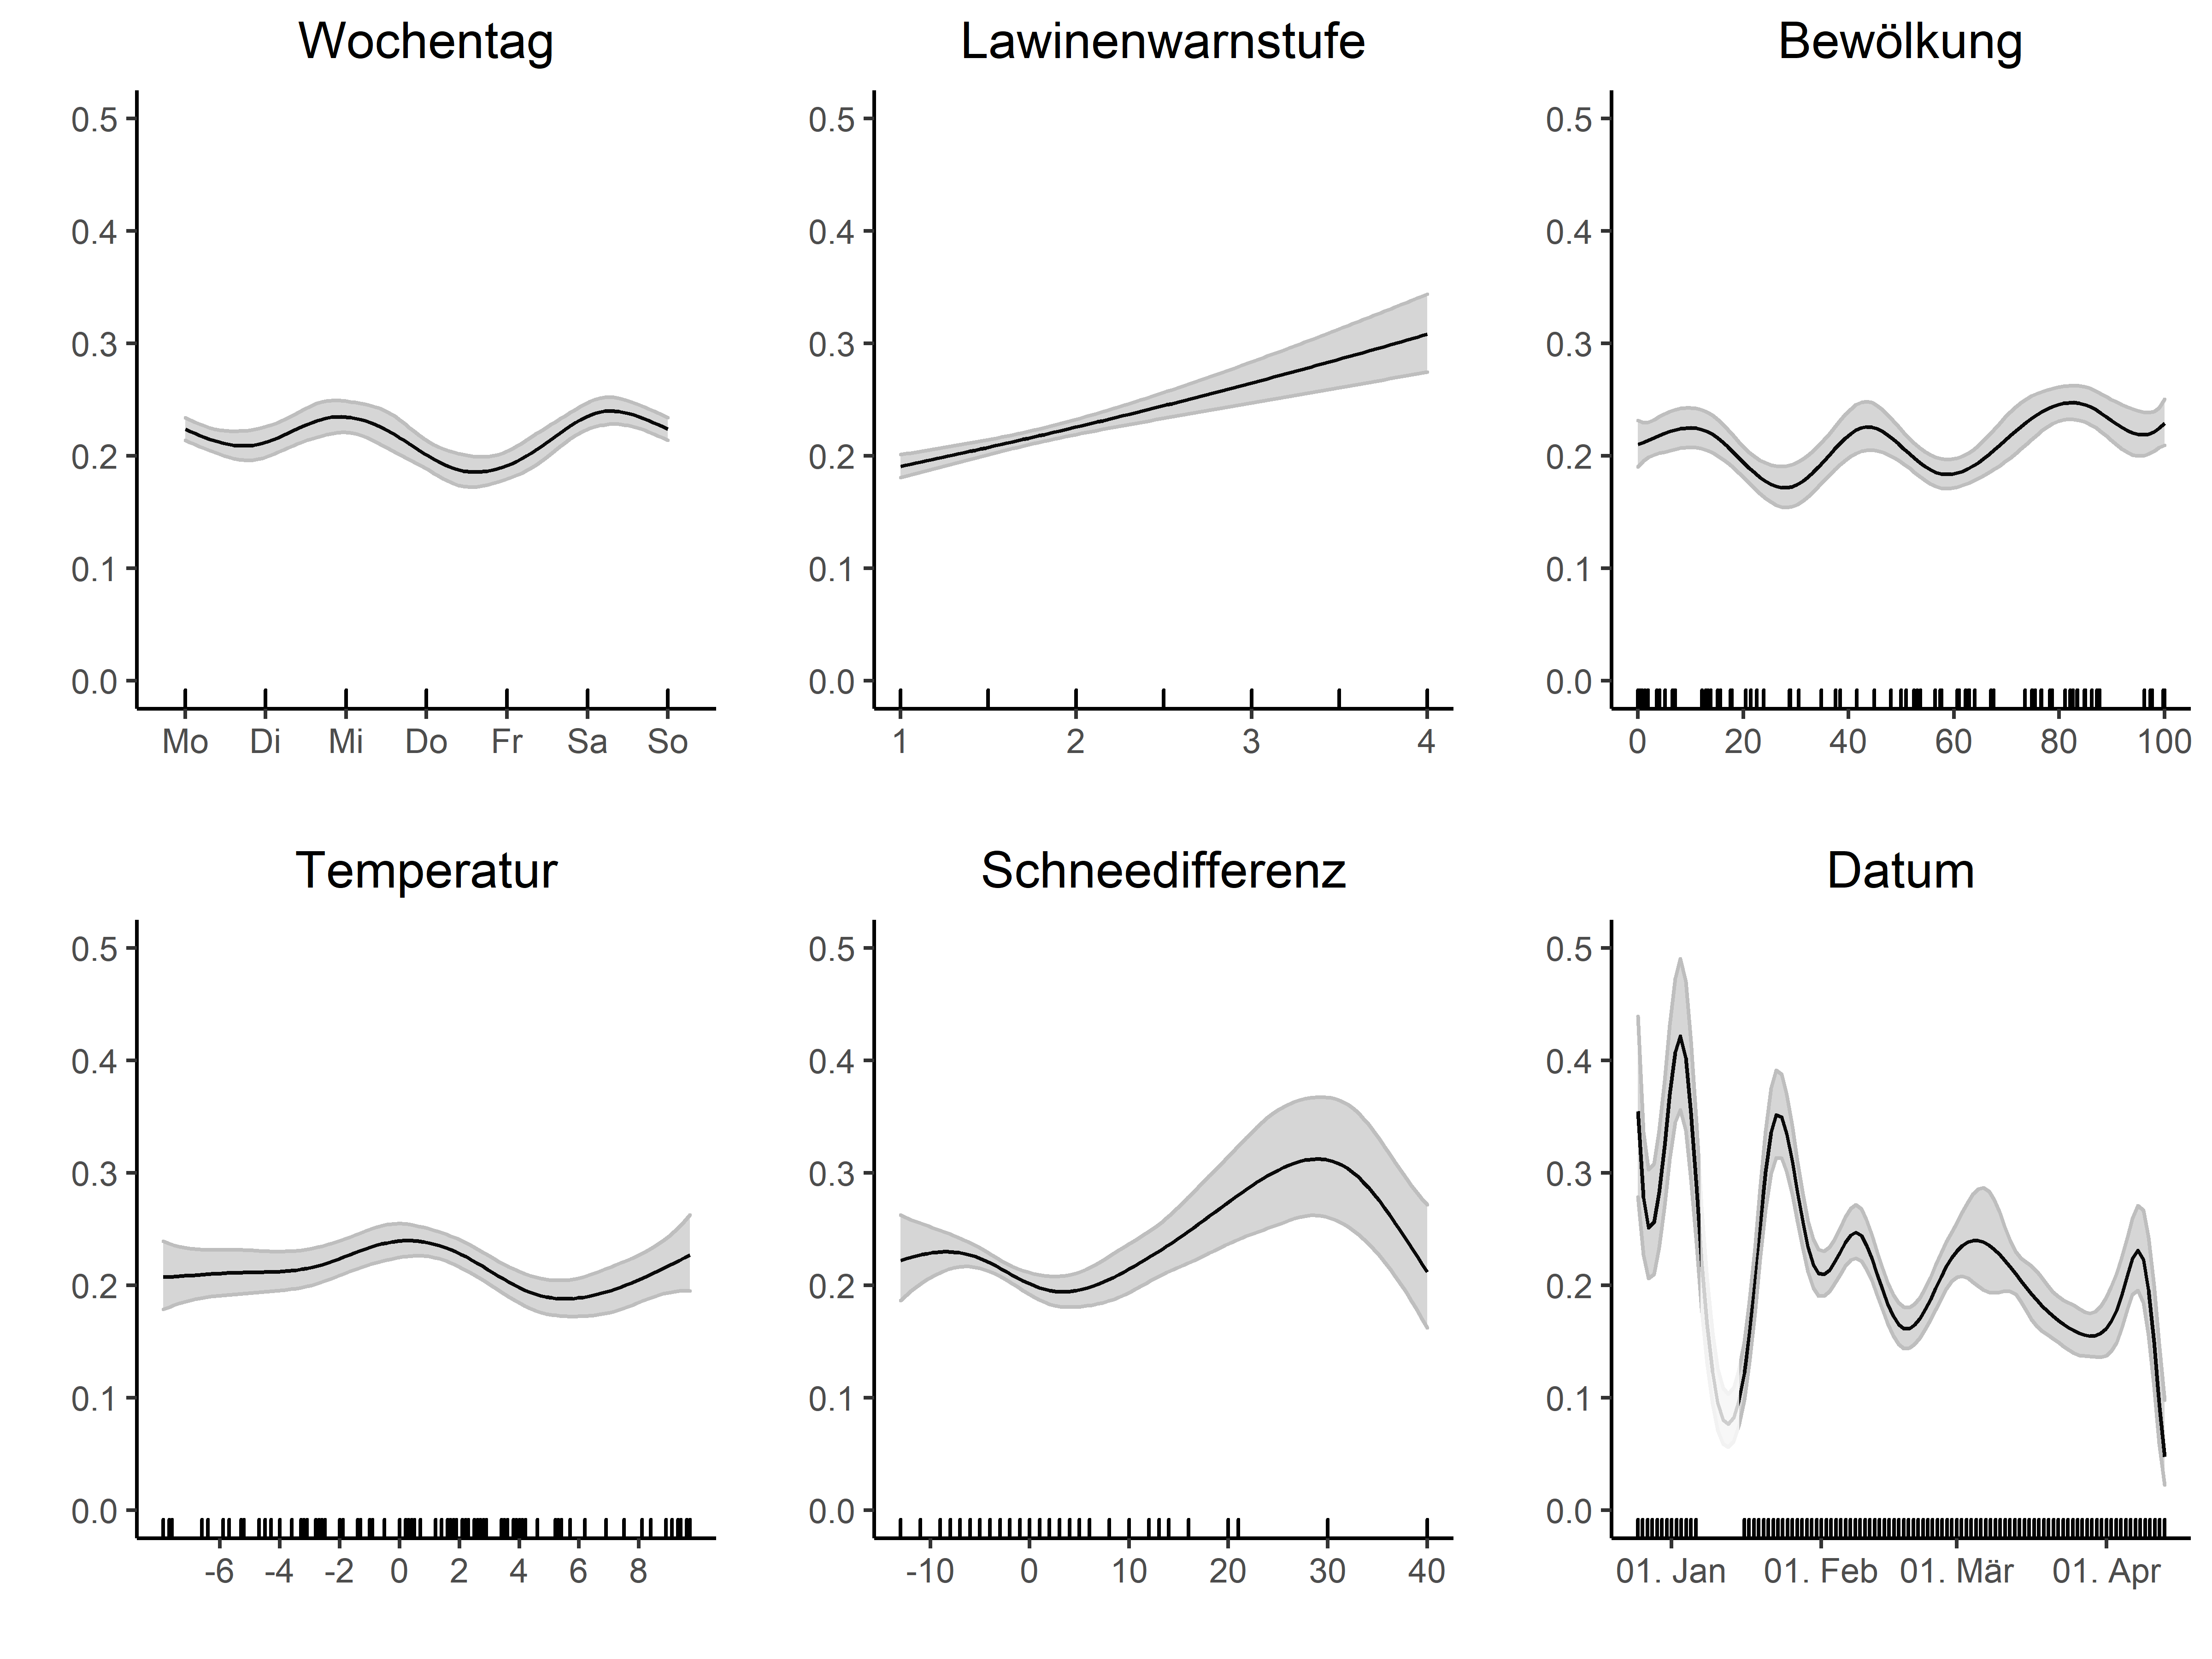
\includegraphics[width=\linewidth]{plots/smooth_day_model}
	\caption{ Die glatten Funktionen der Variablen Wochentag, Lawinenwarnstufe, durchschnittliche Tages-Bewölkung, Temperatur, Schneedifferenz und Datum für das Tagesmodell }
	\label{pic:smooth_day_model}	
\end{figure}
\noindent In Abbildung (\ref{pic:smooth_day_model}) werden die glatten Funktionen der nichtparametrischen Variablen dargestellt. Im Folgenden werden diese einzeln beschrieben.
\subsubsection*{Wochentag:}
An einem Montag, der kein Ferientag ist und an dem alle anderen Kovariablen durchschnittlich sind, liegt der zu erwartende Anteil von Personen mit LVS-Geräten bei etwas über 20\%. Dienstags ist der Anteil etwas geringer und mittwochs höher. Am Donnerstag sinkt dieser auf unter 20\%, um dann bis Samstag auf knapp 25\% anzusteigen. Sonntags ist der Anteil etwas geringer als am Samstag.
\subsubsection*{Lawinenwarnstufe:}
Bei einer Lawinenwarnstufe von 1 ist ein zu erwartender Anteil von Personen mit LVS-Gerät von knapp 20\% zu erkennen. Je höher die Warnstufe desto höher ist auch der zu erwartende Anteil. Bei Lawinenwarnstufe 4 ist ein Anteil von ca. 30\% zu erwarten. Zu beobachten ist, dass das 95\%-Konfidenzintervall ebenfalls breiter wird. Dies lässt sich darauf zurückführen, dass weniger Tage mit hohen Lawinenwarnstufen vorliegen.
\subsubsection*{Durchschnittliche Tages-Bewölkung:}
Bei der glatten Funktion der Variable Bewölkung ist zu beobachten, dass der zu erwartende Anteil von Personen mit LVS-Geräten stark schwankt. Bei einer Bewölkung von 0\% wird ein Anteil von etwas über 20\% erwartet. Der Anteil der LVS-Geräte nimmt bis ca. 10\% Bewölkung zu und fällt bei etwa 30\% Bewölkung auf einen Wert von ungefähr 18\%. Auch danach sind Schwankungen mit Hochpunkten bei ca. 45\% und 85\% Bewölkung ersichtlich. Niedrigere zu erwartende Anteile dagegen erreichen 60\% und 100\% Bewölkung.
\subsubsection*{Temperatur:}
Der zu erwartende Anteil von Personen mit LVS-Geräten liegt bei negativen Temperaturen bei ungefähr 20\%. Nahe dem Nullpunkt ($0^\circ$C) steigt er und fällt dann wieder ab. Bei ca. $5^\circ$C liegt der Anteil erneut bei 20\% und steigt danach wieder an.
\subsubsection*{Schneedifferenz:}
Der zu erwartende Anteil steigt zwischen einer Schneedifferenz von 0 cm und 30 cm von etwa 20\% auf 30\% an. An Tagen mit negativer Schneedifferenz (also weniger Schnee als am Vortag) sinkt der Anteil leicht je näher die Schneedifferenz an 0 cm herankommt. Bei sehr hohen Schneedifferenzen sinkt dann der Anteil wieder. Allerdings zeigt sich dort ein breites Konfidenzintervall. Dies lässt sich durch wenige Tage mit hohen Schneedifferenzen erklären.
\subsubsection*{Datum:}
Der zu erwartende Anteil von Personen mit LVS-Geräten schwankt sehr viel von unter 10\% auf über 40\%. Trotzdem lässt sich eine generelle Abnahme erkennen. Vorsicht ist bei der Interpretation an den fehlenden Tagen geboten, weshalb die Glättung an diesen Tagen transparenter dargestellt wurde.
\subsection{Ergebnisse des Zeitmodells}
Nachfolgend werden die Ergebnisse des Zeitmodells betrachtet. Hier wurden die Messungen nicht nach dem Tag, sondern nach der Minute gruppiert. Insgesamt gibt es n = 19334 Minuten, in denen mindestens eine Messung vorliegt. \\
Der Intercept des Zeitmodells liegt etwas niedriger als der des Tagesmodells, nämlich bei 20,32\%. Der zu erwartende Anteil an einem Ferientag mit ansonsten durchschnittlichen Variablen ist dafür höher und liegt bei 21, 40\%. \\
\begin{figure}[H]
	\centering
	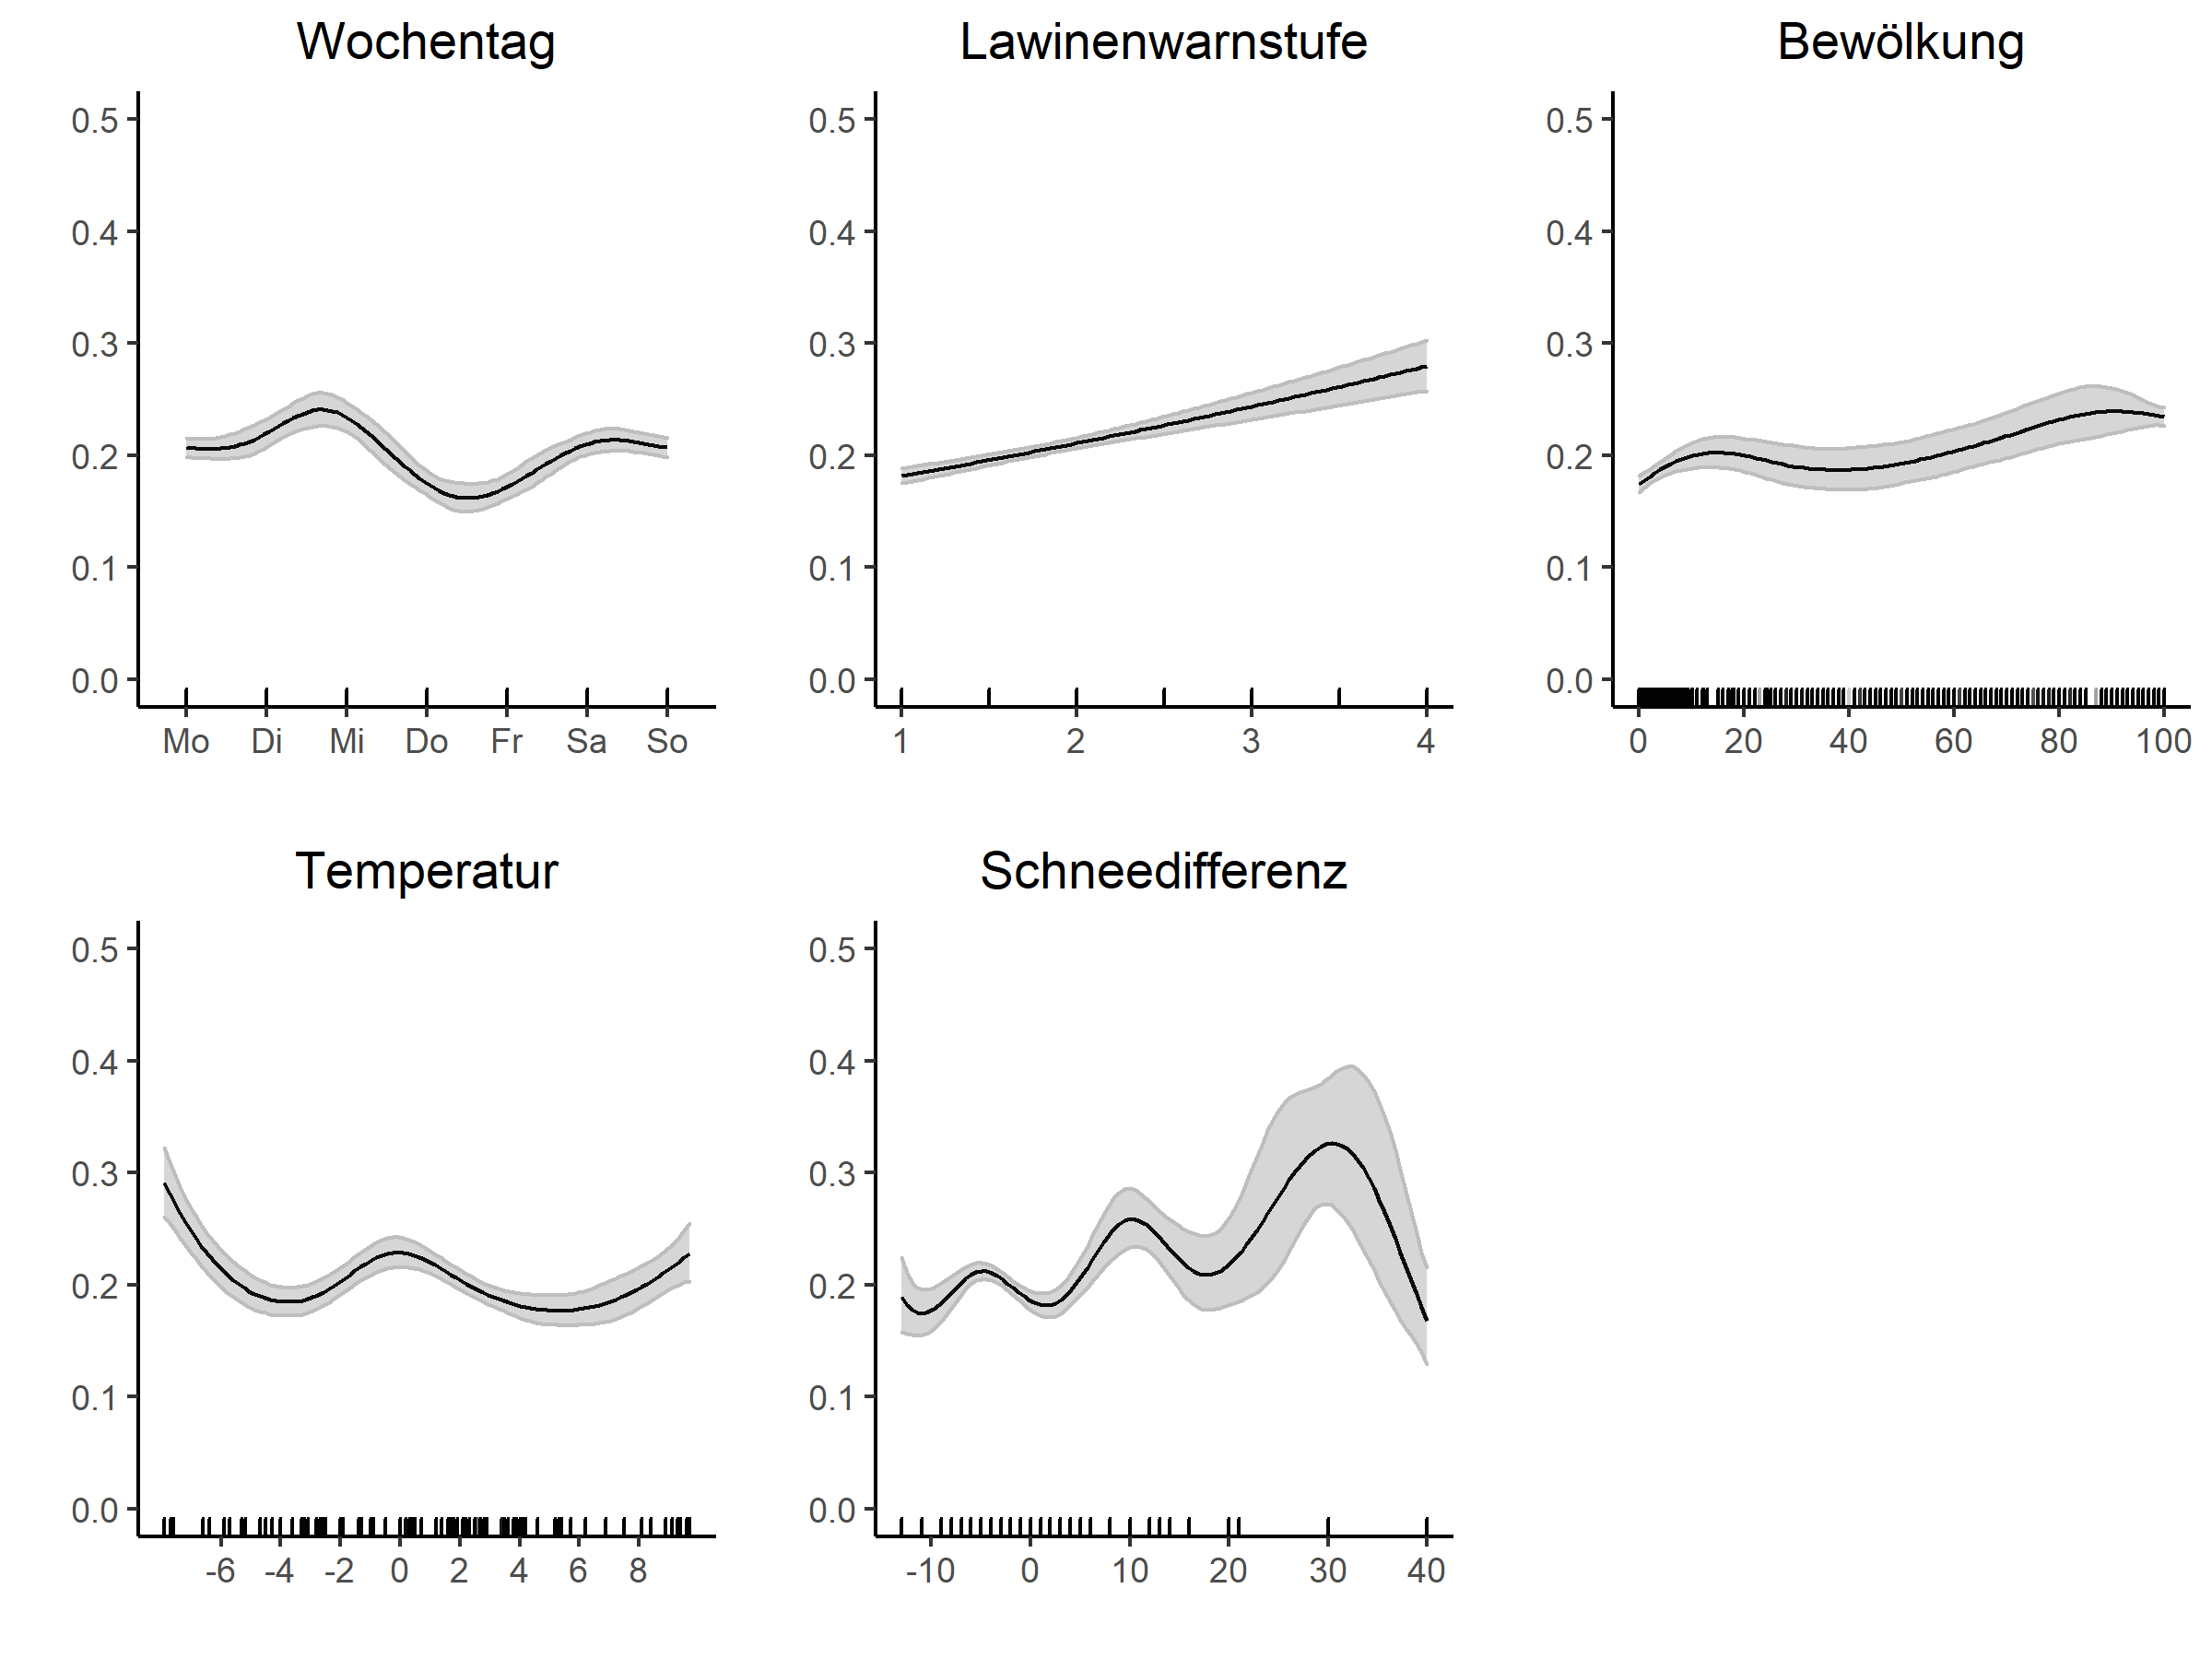
\includegraphics[width=\linewidth]{plots/smooth_time_model}
	\caption{ Die glatten Funktionen der Variablen Wochentag, Lawinenwarnstufe, durchschnittliche Tages-Bewölkung, Temperatur, Schneedifferenz und Datum für das Tagesmodell }
	\label{pic:smooth_time_model}	
\end{figure}
\noindent In Abbildung (\ref{pic:smooth_time_model}) zu sehen sind die glatten Funktionen der nichtparametrischen Variablen (bis auf das Datum und die Uhrzeit der Messungen). Diese werden nun mit den jeweiligen glatten Funktionen des Tagesmodells verglichen. \\
Bei Wochentag und Lawinenwarnstufe ist ein ähnlicher Trend wie beim Tagesmodell zu erkennen. Die Glättung der Variable Bewölkung schwankt deutlich weniger und es lässt sich ein positiver Zusammenhang erkennen. Je bewölkter es ist, desto höher ist der zu erwartende Anteil der Personen mit LVS-Gerät. \\
Auch die glatte Funktion der Temperatur verhält sich ähnlich zum Tagesmodell. Bei Minusgraden ist der zu erwartende Anteil allerdings nicht mehr konstant, sondern nimmt mit sinkender Temperatur zu. Bei der glatten Funktion der Variable Schneedifferenz ist ein Trend zu beobachten. Wie auch beim Tagesmodell steigt der Anteil mit steigender Schneedifferenz. Allerdings schwankt der zu erwartende Anteil deutlich und sinkt nach einer Schneezunahme von 10 cm nochmal ab, bevor er wieder steigt.
\begin{figure}[H]
	\centering
	\includegraphics[width=\linewidth]{plots/time_model_date_time}
	\caption{Die glatte Funktion der Interaktion von Uhrzeit und Datum für das Zeitmodell (Linien stellen Sonnenauf- und untergang dar)}
	\label{pic:time_model_date_time}	
\end{figure}
\noindent In Abbildung (\ref{pic:time_model_date_time}) ist die Glättung der Variablen Uhrzeit und Datum zu erkennen. Über die Saison hinweg kann man eine generelle Abnahme des zu erwartenden Anteils von Personen mit LVS-Gerät erkennen. \\
Betrachtet man die Uhrzeit wird ersichtlich, dass morgens von ungefähr 7:00 bis 11:00 Uhr ein besonders hoher zu erwartender Anteil von bis zu 40\% zu beobachten ist. Abends von 19:00 bis 22:00 ist ein geringer Anstieg des Anteils erkennbar. Das zu diesen Uhrzeiten ein erhöhter Anteil von Personen mit LVS-Gerät zu erwarten ist ändert sich auch im Verlauf der Saison kaum und scheint nicht mit der Uhrzeit des Sonnenauf- und -untergangs zusammenzuhängen.

\subsection{Signifikanz}
Neben dem Verlauf der glatten Funktionen werden auch die Signifikanzen der Variablen für beide Modellen betrachtet. \\
Zu beobachten ist, dass sich die Signifikanzen der einzelnen Variablen (auf einem 5\%-Signifikanzniveau) zwischen den Modellen stark unterscheiden. Während beim Tagesmodell nur der Intercept, das Datum und die Lawinenwarnstufe signifikant sind, so sind beim Zeitmodell alle Variablen, bis auf Ferientag, und der Intercept signifikant. \\
Ob eine Variable signifikant ist, also ob der Einfluss der Kovariable auf die Zielvariable mehr als nur zufällig ist, hängt auch von der Anzahl der Beobachtungen (n) ab. Es ist nicht au"ser Acht zu lassen, dass das Tagesmodell n = 101 Beobachtungen aufweist, wohingegen das Zeitmodell n = 19334 Beobachtungen hat.

\chapter{Messfehleranalyse}
\label{chap:Messfehleranalyse}
Wie bereits zuvor erwähnt, haben die Projektpartner festgestellt, dass die Checkpoints in ihrer Messung Messfehler haben. \\
Messfehler sind Abweichungen der erhobenen Daten vom wahren Wert. In unserem Fall bedeutet das, dass die Checkpointmessungen nicht exakt den vorbeigehenden Personen mit oder ohne LVS-Gerät entsprechen, somit ist eine mögliche Unter-/Überschätzung des Anteils an LVS-Geräten vorhanden. Dabei können Messfehler verschiedener Art vorkommen, die jeweils eigene Ursachen haben, und so die Stärke und Richtung der Fehlschätzung unterschiedlich beeinflussen. \\
Im folgenden Teil werden erst von den Projektpartnern gesammelte Daten über die Genauigkeit der Checkpointmessungen an zwei Tagen untersucht und danach (unter anderem) daraus verschiedene Szenarien für mögliche Messfehler erstellt. Anhand des jeweiligen Szenarios werden Messungen aus dem originalen Datensatz ergänzt oder entfernt und es wird verglichen, inwiefern sich die Ergebnisse unserer zwei Modelle für die gewählten Szenarien unterscheiden.

\section{Messfehler Beschreibung}
Um die Schwere und Art der Messfehler zu untersuchen, wurde eine Gruppe von Studenten mehrmals zum Aufstiegsort geschickt. Unter Anderem wurden dabei verschiedene Tests angestellt, z.B. wurde die Erfassung der Personen abhängig von unterschiedlichen Entfernungen und Winkeln zum Checkpoint untersucht oder man ließ einen Hund mehrmals am Checkpoint vorbeilaufen und markierte, wann dieser vom Checkpoint registriert wurde und wann nicht. Für die folgende Analyse werden Daten benutzt, die von einer manuellen Zählung einer solchen Gruppe von Studenten am 27.02. und 28.02.2020 stammen. Genauer gesagt fanden die Zählungen zu drei unterschiedlichen Zeiträumen statt: am 27.02. von 10:32 bis 12:58, am 28.02. von 10:38 bis 12:26 und von 14:40 bis 16:50. \\
Dabei wurde eingetragen, wie viele mögliche Kontakte zu jeder Minute am Checkpoint vorbeigegangen sind. Zudem werden die Kontakte auf zwei verschiedene Arten unterschieden. Einerseits gibt es eine Unterscheidung zwischen „Skitourengeher“, die eigentlich zu interessierende Art von Besuchern mit eventuellen LVS-Geräten, und „andere Kontakte“, also andere Besucher wie Spaziergänger oder z.B. ein Hund. Andererseits wird zusätzlich zwischen „erfassten“ und „nicht erfassten“ Kontakten unterschieden, wobei ein Kontakt als erfasst gilt, wenn er augenscheinlich vom Checkpoint erkannt und registriert wurde.\\
Wichtig zu erwähnen ist, dass bei der manuellen Zählung keine Unterscheidung zwischen Besuchern mit und ohne LVS-Gerät gemacht wurde. Zusätzlich zu den manuellen Zählungen liegen die tatsächlich von den Checkpoints erhobenen Messungen zur Saison 19/20 vor, wobei einer der Checkpoints früh in der Saison ausgefallen ist und zu den zwei Tagen der manuellen Zählungen somit nur ein Checkpoint aktiv war.

\section{Messfehler deskriptive Analyse}
Die Anzahl der in der manuellen Zählung eingetragenen Kontakte beträgt insgesamt 208. Davon sind 122 Skitourengeher und 86 andere Kontakte. Als erfasst vom Checkpoint wurden 161 Kontakte eingetragen, als nicht erfasst somit 47. \\
Da die angegebenen Uhrzeiten in der manuellen Zählung und der tatsächlichen Registrierung im Checkpoint voneinander abweichen, werden beim genaueren Vergleich von Erfassungen und Nichterfassungen nur die Daten der manuellen Zählung hergenommen. Für den gesamten Zeitraum der manuellen Zählung kann man jedoch die tatsächlich vom Checkpoint eingetragene Anzahl an erfassten Kontakten hernehmen, die mit 170 etwas höher ist als die 161 von den Studenten angegebenen Nichterfassungen. Für die Berechnung der Unterschätzung insgesamt wird deshalb die Anzahl der vom Checkpoint gemessenen Kontakte, also 170, mit den insgesamt durch die manuelle Zählung festgehaltenen Kontakten, also 208, verglichen. Damit kommt man auf eine allgemeine Unterschätzung des Checkpoints von ca. 22\%. Hierbei wird \glqq Unterschätzung \grqq definiert als der Anteil an vorhandenen Messungen, die man dem Checkpoint hinzufügen müsste, um auf den wahren Wert der vorbeigehenden Kontakte zu bekommen. In unserem Fall müsste man dem Checkpoint ca. 22\% von 170 erfassten Kontakten hinzufügen, um auf den wahren Wert von 208 Kontakten zu kommen. \\
Für die Berechnung der Unterschätzung wurden keine Messungen aus den manuellen Zählungen entfernt. Insbesondere auch keine Fälle, zu denen angegeben war, dass das Gerät durch fälschliche Messungen wie Mehrfacherfassungen einer Person den wahren Wert überschätzt. In diesem Sinne ist die berechnete Unterschätzung keine „reine“ Unterschätzung sondern die Unterschätzung für alle gemessenen Beobachtungen.
Um zu testen, wie genau die Erfassung des Checkpoints bei größeren Gruppen an vorbeigehenden Kontakten funktioniert, wurde eine Untersuchung des Anteils an erfassten Kontakten in Abhängigkeit von Gruppengröße durchgeführt. Als Gruppe zählen hierbei alle Kontakte, die zur selben Uhrzeit in der manuellen Zählung vermerkt wurden. Sind also beispielsweise um 15:23 vier Kontakte in der manuellen Zählung vermerkt, so gilt dies als Gruppe von vier Personen. In den Daten kommen jeweils mehrere Gruppen in einer Grö"se von 1 bis 5 und eine Gruppe von 8 Kontakten vor. \\
\begin{figure}[H]
	\centering
	\includegraphics[width=\linewidth]{plots/erf_gruppe_rel_plot}
	\caption{ }
	\label{pic:erf_gruppe_rel_plot}	
\end{figure}
\noindent Wie man in der Abbildung (\ref{pic:erf_gruppe_rel_plot})sieht, schwankt der Anteil von Nichterfassungen an allen Messungen bei den fünf kleineren Gruppengrö"sen um einen Wert von 18\%, der einer Unterschätzung von 22\% entspricht. (0.18/0.82=0.22) In der Achtergruppe ist der Anteil von Nichterfassungen allerdings über 50\%, d.h. es wurden in dieser Gruppe mehr Kontakte vom Checkpoint nicht erkannt als erkannt.

\section{Messfehlerszenarien im Vergleich}
\subsection{Szenarien im Tagesmodell}
\begin{table}[htbp]
	\centering
	\caption{Tabelle für das Original, Szenario 1 (Generelle Unterschätzung von 22\%), Szenario 2 (Unterschätzung nach Gruppengrö”se), Szenario 3 (Nächtliche Überschätzung) und Szenario 4 (Unterschätzung nach Temperatur) für das Tagesmodell}
	\begin{adjustbox}{max width=\textwidth}
	\begin{tabular}{l|ccc|ccc|ccc|ccc|ccc|}
		\multicolumn{1}{r}{} & 
		\multicolumn{3}{c}{Original} & 
		\multicolumn{3}{c}{Szenario 1} & 
		\multicolumn{3}{c}{Szenario 2} & 
		\multicolumn{3}{c}{Szenario 3} & 
		\multicolumn{3}{c}{Szenario 4} \\
		& Koeffizient & p-Wert &       & Koeffizient & p-Wert &       & Koeffizient & p-Wert &       & Koeffizient & p-Wert &       & Koeffizient & p-Wert &  \\
		\cmidrule{2-16}    (Intercept) & 0.217 & <2e-16 & ***   & 0.158 & <0.01 & ***   & 0.174 & <2e-16 & ***   & 0.232 & <2e-16 & ***   & 0.172 & <2e-16 & *** \\
		Ferientag & 0.197 & 0.748 &       & 0.162 & 0.94  &       & 0.156 & 0.701 &       & 0.216 & 0.81  &       & 0.159 & 0.785 &   \\
		s(Datum) &       & 0.005 & **    &       & <0.01 & ***   &       & 0.005 & **    &       & 0.02  & *     &       & 0.007 & ** \\
		s(Lawinengefahr) &       & 0.030 & *     &       & 0.03  & *     &       & 0.035 & *     &       & 0.06  & .     &       & 0.030 & * \\
		s(Wochentag) &       & 0.198 &       &       & 0.05  & .     &       & 0.177 &       &       & 0.15  &       &       & 0.207 &   \\
		s(Temperatur) &       & 0.713 &       &       & 0.70  &       &       & 0.681 &       &       & 0.69  &       &       & 0.639 &   \\
		s(Bewölkung) &       & 0.371 &       &       & 0.85  &       &       & 0.278 &       &       & 0.24  &       &       & 0.365 &   \\
		s(Schneedifferenz) &       & 0.635 &       &       & 0.48  &       &       & 0.647 &       &       & 0.72  &       &       & 0.651 &   \\
		\cmidrule{2-16}    \end{tabular}%
	\end{adjustbox}
	\label{tab:Szenarien im Tagesmodell}%
\end{table}%

\noindent Tabelle (\ref{tab:Szenarien im Tagesmodell}) zeigt im Tagesmodell die Werte für die Koeffizienten von Intercept und Ferientag, die p-Werte und Signifikanzen für alle Kovariablen für den originalen Datensatz und jedes Messfehlerszenario im Vergleich. \\
Da in den Szenarien nur Beobachtungen ohne LVS-Gerät hinzugefügt bzw. entfernt werden, sinken bzw. steigen die Koeffizienten für die zwei parametrischen Variablen entsprechend. Szenario 1 mit genereller Unterschätzung hat die höchste Menge an hinzugefügten Beobachtungen, deswegen ist der Intercept, also der Anteil an Messungen mit LVS-Geräten bei konstant gehaltenen Kovariablen und keinem Ferientag, mit einem Wert von 15,8\% am geringsten. Szenario 3 mit nächtlicher Überschätzung ist das einzige Szenario, bei dem Beobachtungen entfernt werden, deswegen steigt hier der Koeffizient für den Intercept auf einen Wert von 23,2\%. Analog gelten die Aussagen für den Anteil an Ferientagen bei konstant gehaltenen Kovariablen. Bei der generellen Unterschätzung ist der Wert für Ferientage mit 16,2\% höher als der Wert für den Intercept. \\
Bei einem Signifikanzniveau von 5\% haben nur der Intercept und das Datum bei allen Szenarien wie im Original einen statistisch signifikanten Zusammenhang mit dem Anteil an LVS-Geräten. Die Kovariable für Lawinengefahr hat im Original und bei jedem Szenario außer der nächtlichen Überschätzung einen statistisch signifikanten Zusammenhang. Alle anderen Kovariablen, als für Ferientag, Bewölkung, Wochentag, Temperatur, Bewölkung und Schneedifferenz, haben wie im Original keinen statistischen Zusammenhang mit dem Anteil auf dem gewählten Signifikanziveau. \\
\begin{figure}[H]
	\centering
	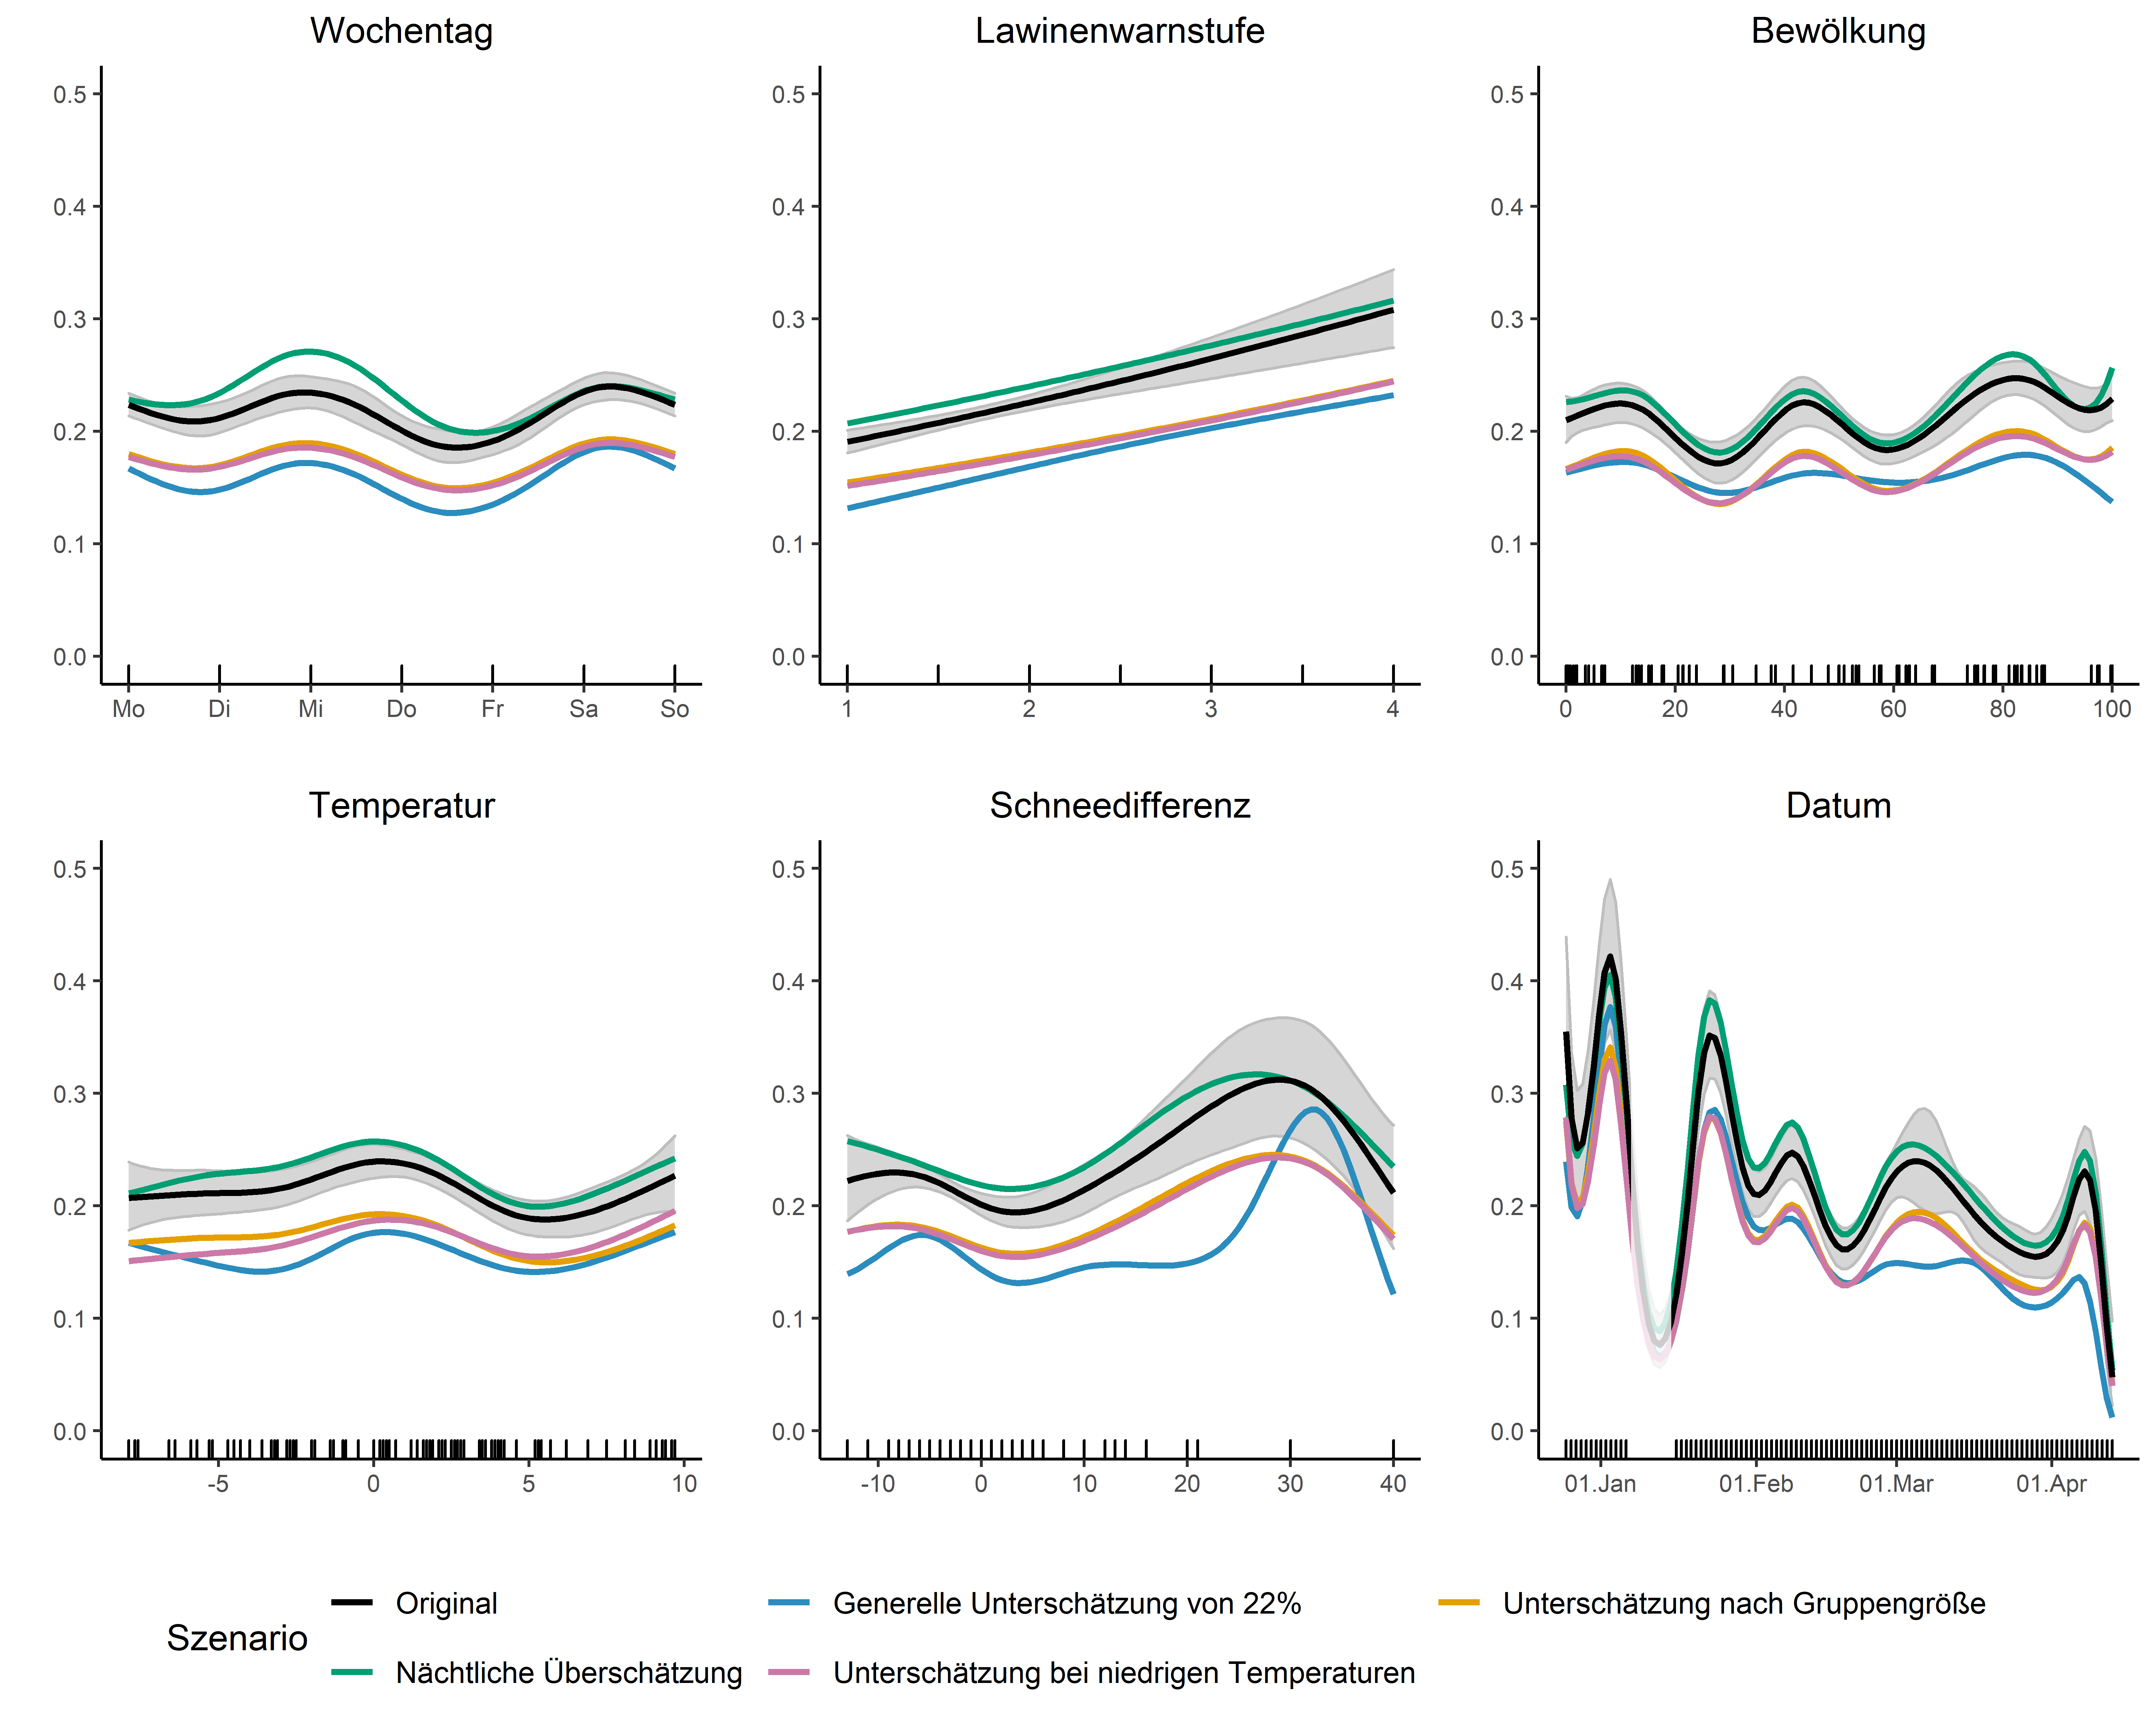
\includegraphics[width=\linewidth]{plots/day_model_comparison_plots}
	\caption{ Die glatten Funktionen der Variablen Wochentag, Lawinenwarnstufe, durchschnittliche Tages-Bewölkung, Temperatur, Schneedifferenz und Datum für das Tagesmodell für die verschiedenen Szenarien}
	\label{pic:day_model_comparison_plots}	
\end{figure}
\noindent Abbildung (\ref{pic:day_model_comparison_plots}) zeigt im Tagesmodell den Zusammenhang zwischen Anteil an LVS-Geräten und allen nonparametrischen Kovariablen im Original und den verschiedenen Messfehlerszenarien. \\
Es lässt sich anhand von Abbildung (\ref{pic:day_model_comparison_plots}) feststellen, dass die Zusammenhänge der einzelnen Kovariablen mit dem Anteil an LVS-Geräten für alle Szenarien zumeist einen ähnlichen Verlauf nehmen wie im Original. So hat die glatte Funnktion z.B. für den Wochentag bei jedem Szenario wie im Original höhere Werte für Montag, Mittwoch und Samstag als für Dienstag, Donnerstag oder Freitag. Auch für die anderen Kovariablen unterscheidet sich der Verlauf des Zusammenhangs insbesondere für Szenarien 2 bis 4 nur geringfügig vom Original. \\
Einzig in Szenario 1, der generellen Unterschätzung, sind an mehreren Stellen grö"ssere Unterschiede zu bemerken. So schwankt der Anteil im Zusammenhang mit der Bewölkung  weniger stark als im Original und den anderen Szenarien. Für niedrige Temperaturen bis -3 Grad sinkt der Anteil im Gegensatz zu den anderen Szenarien, verläuft danach aber ähnlich. Bei einer Schneedifferenz von 5 bis 20 cm steigt der Anteil geringer als in den anderen Szenarien bis nur ca. 15\%, für Werte zwischen 20 und 32 cm dagegen steigt der Anteil in Szenario 1 deutlich stärker und sinkt danach auch deutlich stärker ab als in den anderen Szenarien, mit einem Höchstwert von ca. 28\%. \\
Wie schon erwähnt ist die Unsicherheit in diesem Bereich allerdings erhöht, da nur wenige Tage mit hohen Werten für die Schneedifferenz vorkommen. Beim Datum unterscheidet sich Szenario 1 im Bereich vom 01. März bis zum15. März, da der Anteil dort fast konstant bei ca. 15\% liegt und nicht wie in den anderen Szenarien ansteigt und wieder abfällt.

\subsection{Szenarien im Zeitmodell}
\begin{table}[htbp]
	\centering
	\caption{Tabelle für das Original, Szenario 1 (Generelle Unterschätzung von 22\%), Szenario 2 (Unterschätzung nach Gruppengrö”se), Szenario 3 (Nächtliche Überschätzung) und Szenario 4 (Unterschätzung nach Temperatur) für das Zeitmodell}
	\begin{adjustbox}{max width=\textwidth}
	\begin{tabular}{l|ccc|ccc|ccc|ccc|ccc|}
		\multicolumn{1}{r}{} & \multicolumn{3}{c}{Original} & \multicolumn{3}{c}{Szenario 1} &
		\multicolumn{3}{c}{Szenario 2} & 
		\multicolumn{3}{c}{Szenario 3} & 
		\multicolumn{3}{c}{Szenario 4} \\
		& Koeffizient & p-Wert &       & Koeffizient & p-Wert &       & Koeffizient & p-Wert &       & Koeffizient & p-Wert &       & Koeffizient & p-Wert &  \\
		\cmidrule{2-16}    (Intercept) & 0.203 & <2e-16 & ***   & 0.127 & <2e-16 & ***   & 0.163 & <2e-16 & ***   & 0.218 & <2e-16 & ***   & 0.119 & <2e-16 & *** \\
		Ferientag & 0.214 & 0.2   &       & 0.126 & 0.9   &       & 0.170 & 0.3   &       & 0.229 & 0.2   &       & 0.122 & 0.5   &   \\
		s(Datum) & x     & <2e-16 & ***   & x     & <2e-16 & ***   & x     & <2e-16 & ***   & x     & <2e-16 & ***   & x     & <2e-16 & *** \\
		s(Lawinengefahr) & x     & 6.00E-13 & ***   & x     & <2e-16 & ***   & x     & 5.00E-13 & ***   & x     & 1.00E-12 & ***   & x     & <2e-16 & *** \\
		s(Wochentag) & x     & 2.00E-10 & ***   & x     & 3.00E-15 & ***   & x     & 6.00E-10 & ***   & x     & 6.00E-10 & ***   & x     & 1.00E-10 & *** \\
		s(Temperatur) & x     & 5.00E-10 & ***   & x     & <2e-16 & ***   & x     & 4.00E-10 & ***   & x     & 1.00E-08 & ***   & x     & 1.00E-10 & *** \\
		s(Bewölkung) & x     & 8.00E-16 & ***   & x     & 5.00E-13 & ***   & x     & 4.00E-16 & ***   & x     & 5.00E-16 & ***   & x     & <2e-16 & *** \\
		s(Schneedifferenz) & x     & 6.00E-08 & ***   & x     & 7.00E-09 & ***   & x     & 2.00E-08 & ***   & x     & 1.00E-07 & ***   & x     & 5.00E-08 & *** \\
		\cmidrule{2-16}    \end{tabular}%
	\end{adjustbox}
	\label{tab:Szenarien im Zeitmodell}%
\end{table}%

\noindent Tabelle (\ref{tab:Szenarien im Zeitmodell}) zeigt im Zeitmodell die Werte für die Koeffizienten von Intercept und Ferientag, die p-Werte und Signifikanzen für alle Kovariablen für den originalen Datensatz und jedes Messfehlerszenario im Vergleich. \\
Ähnlich wie beim Tagesmodell verhalten sich die Koeffizienten für den Intercept und Ferientag. In den Szenarien mit Unterschätzung sinken beide Anteile im Vergleich zum Original bei einem Tiefstwert von 12,7\% für den Intercept bei der generellen Unterschätzung und einem erhöhten Wert von 21,8\% beim Szenario der nächtlichen Überschätzung, analog für den Anteil an Ferientagen. Bei der generellen Unterschätzung ist der Anteil an Ferientagen mit 12,6\% geringer ist als an Tagen, die keine Ferientage sind. \\
Wie im Original sind in allen Szenarien alle Variablen bis auf Ferientag statistisch signifikant. \\
\begin{figure}[H]
	\centering
	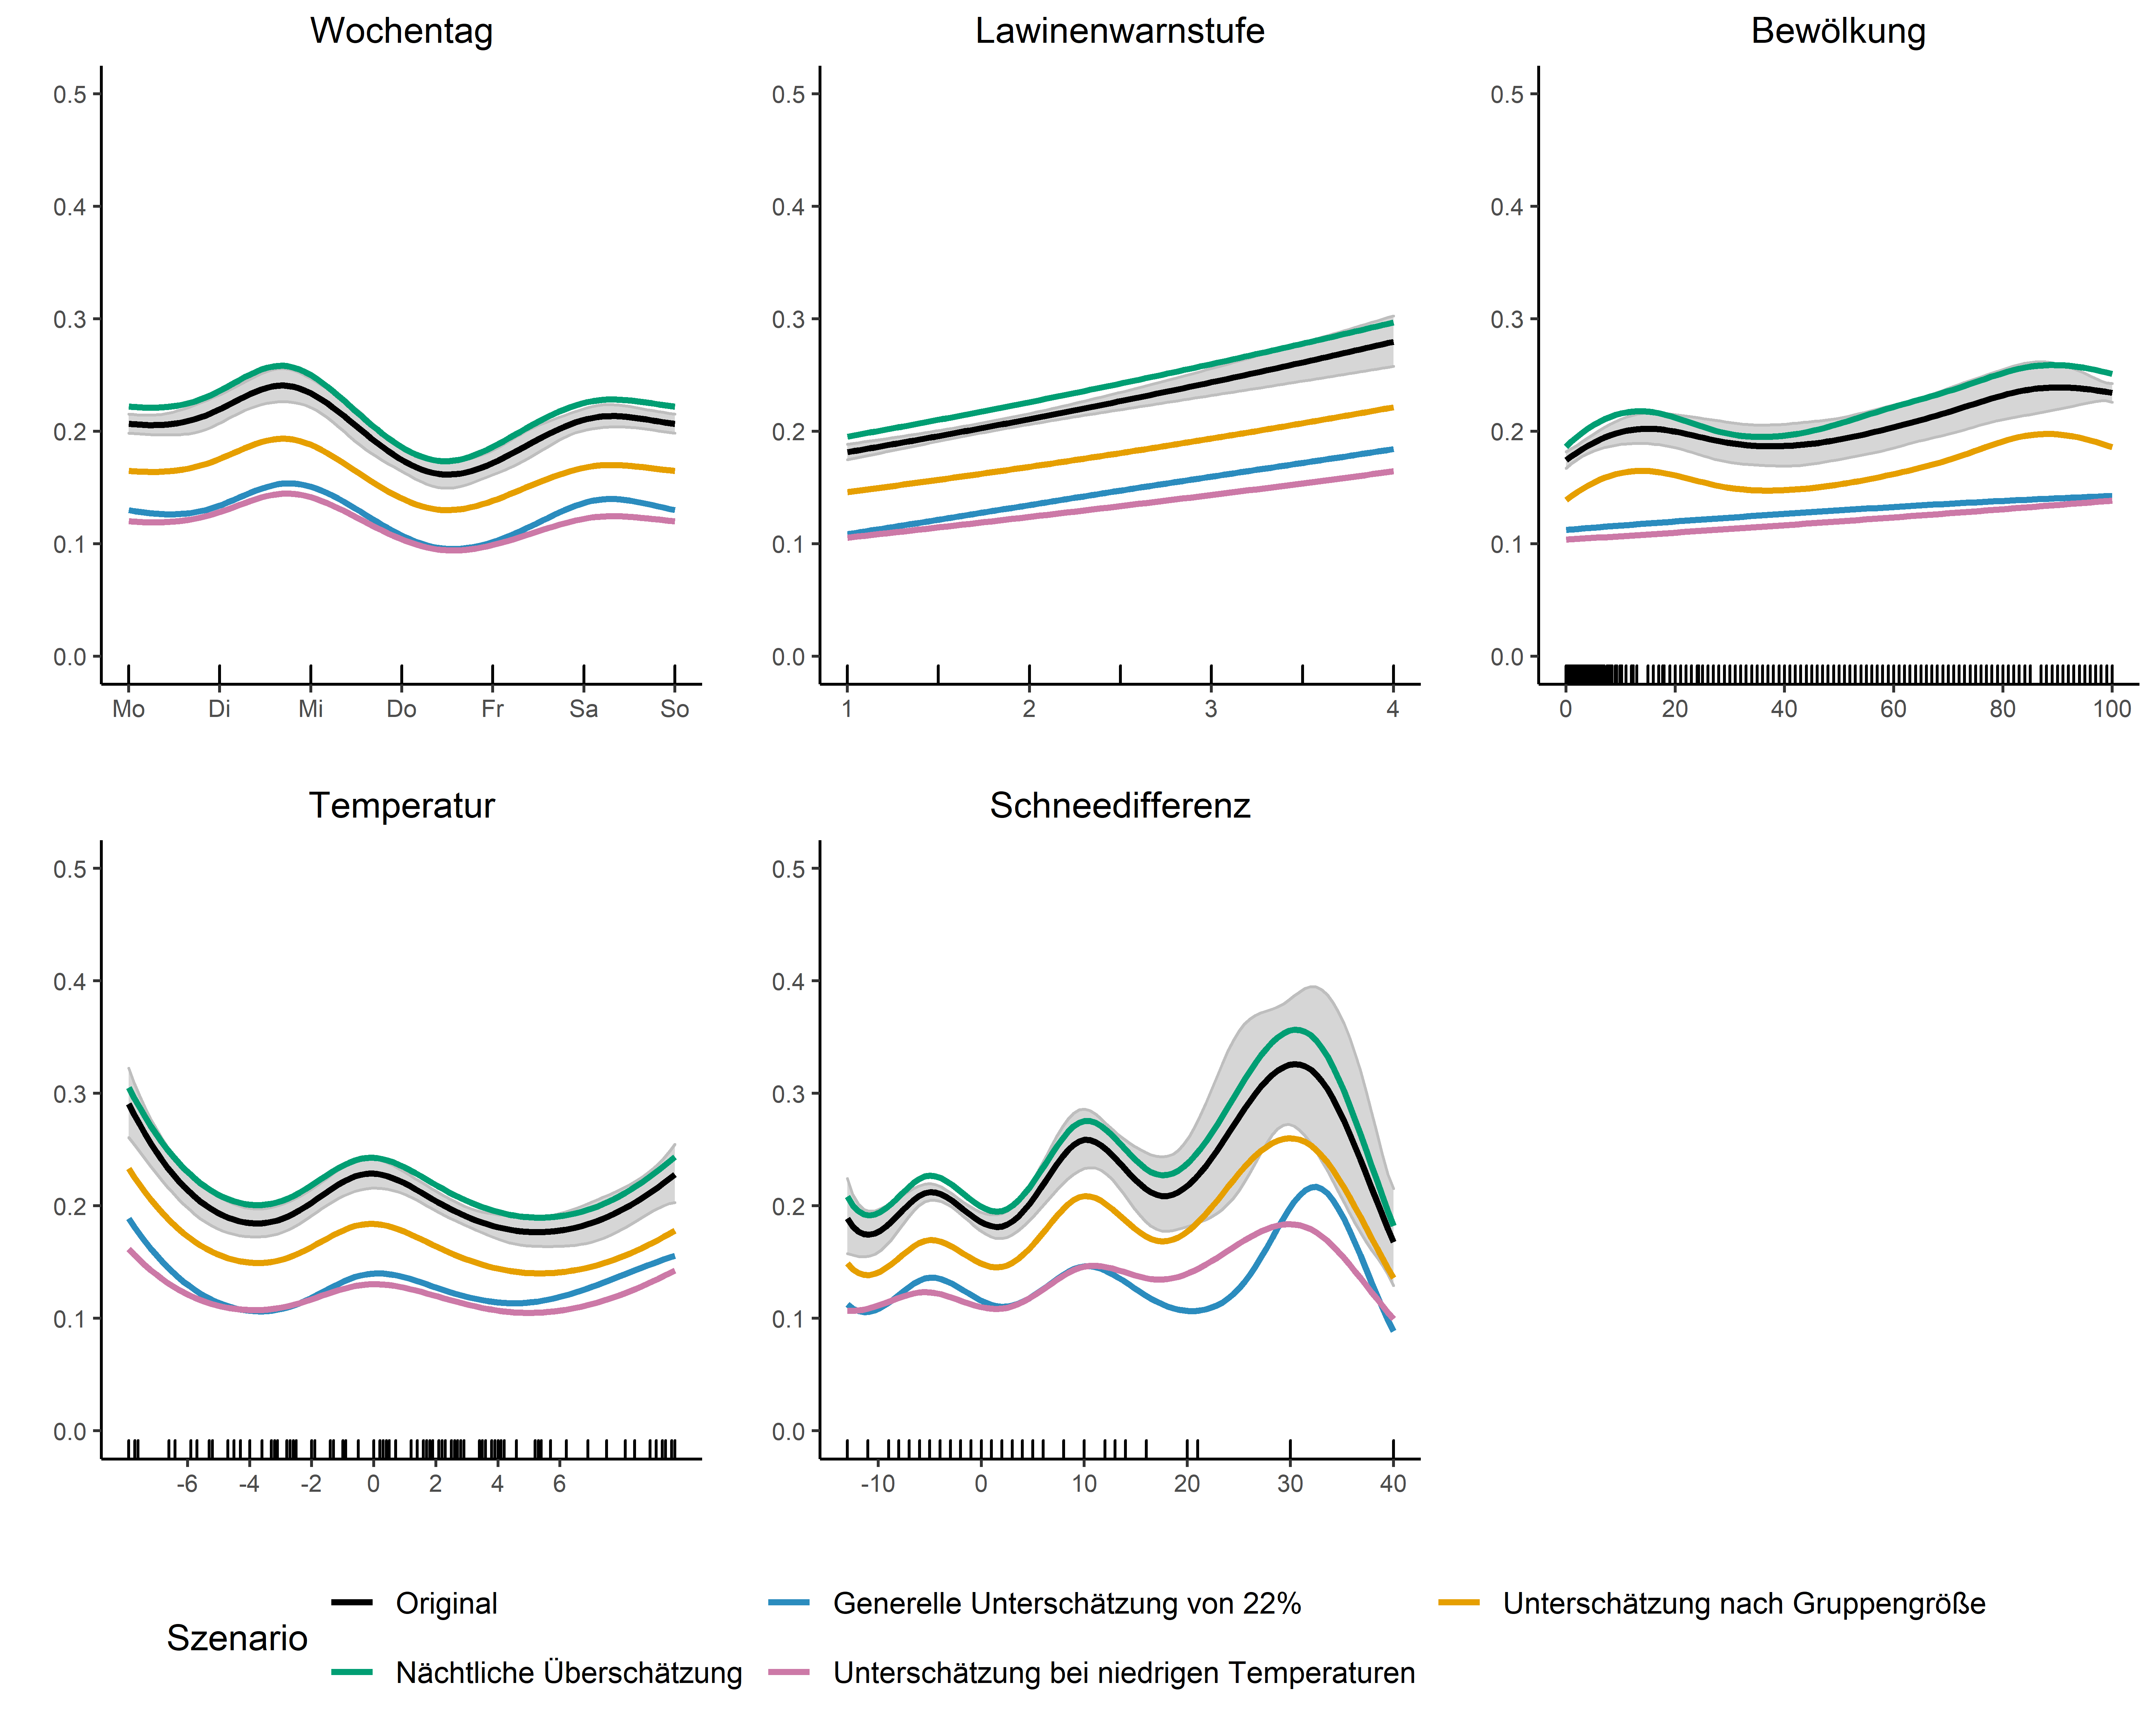
\includegraphics[width=\linewidth]{plots/time_model_comparison}
	\caption{ Die glatten Funktionen der Variablen Wochentag, Lawinenwarnstufe, durchschnittliche Tages-Bewölkung, Temperatur, Schneedifferenz für das Zeitmodell für die verschiedenen Szenarien}
	\label{pic:time_model_comparison}	
\end{figure}
\noindent Die Abbildung (\ref{pic:time_model_comparison}) zeigt im Zeitmodell den Zusammenhang zwischen Anteil an LVS-Geräten und allen nonparametrischen Kovariablen im Original und den verschiedenen Messfehlerszenarien. \\
Wie im Tagesmodell verlaufen die Zusammenhänge der einzelnen Kovariablen mit dem Anteil an LVS-Geräten bei allen Szenarien zumeist ähnlich zum Original. Größere Unterschiede bestehen bei der Bewölkung, wo für das Szenario mit genereller Unterschätzung und einer Unterschätzung bei niedrigen Temperaturen ein konstanter Anstieg bei wachsender durchschnittlicher Bewölkung zu beobachten ist, und bei der Schneedifferenz, wo im Bereich von 10 bis 20 cm der Anteil im Szenario mit Unterschätzung bei niedrigen Temperaturen verhältnismäßig weniger Schwankungen unterliegt. \\
Auffällig ist, dass der Anteil bei Werten für die Schneedifferenz von 20 cm und mehr für das Original und Szenarien 2 bis 4 nun im Vergleich zum Tagesmodell stärker ansteigt und wieder sinkt und somit dem Verlauf von Szenario 1 ähnlicher ist.

\section{Szenario mit steigender genereller Unterschätzung}
Für das Szenario mit genereller Unterschätzung wird im obigen Vergleich eine Unterschätzung von 22\% angenommen. \\
Im Folgenden wird verglichen, wie sich die Ergebnisse der beiden Modelle für unterschiedliche Werte für die allgemeine Unterschätzung verhalten.

\subsection{Szenario 1 im Tagesmodell}

\begin{table}[htbp]
	\centering
	\caption{Add caption}
	\begin{adjustbox}{max width=\textwidth}
	\begin{tabular}{l|ccc|ccc|ccc|ccc|}
		\multicolumn{1}{r}{} & \multicolumn{3}{c}{Original} & \multicolumn{3}{c}{10\%} & \multicolumn{3}{c}{20\%} & \multicolumn{3}{c}{30\%} \\
		& Koeffizient & p-Wert &       & Koeffizient & p-Wert &       & Koeffizient & p-Wert &       & Koeffizient & p-Wert & \multicolumn{1}{c}{} \\
		\cmidrule{2-13}    (Intercept) & 0.217 & <2e-16 & ***   & 0.182 & <2e-16 & ***   & 0.162 & <2e-16 & ***   & 0.145 & <2e-16 & *** \\
		Ferientag & 0.197 & 0.748 &       & 0.181 & 0.984 &       & 0.164 & 0.97  &       & 0.149 & 0.94  &   \\
		s(Datum) &       & 0.005 & **    &       & 0.003 & **    &       & <1e-03 & ***   &       & <1e-03 & *** \\
		s(Lawinengefahr) &       & 0.030 & *     &       & 0.011 & *     &       & 0.02  & *     &       & 0.02  & * \\
		s(Wochentag) &       & 0.198 &       &       & 0.117 &       &       & 0.08  & .     &       & 0.03  & * \\
		s(Temperatur) &       & 0.713 &       &       & 0.720 &       &       & 0.69  &       &       & 0.75  &   \\
		s(Bewölkung) &       & 0.371 &       &       & 0.814 &       &       & 0.89  &       &       & 0.82  &   \\
		s(Schneedifferenz) &       & 0.635 &       &       & 0.527 &       &       & 0.42  &       &       & 0.40  &   \\
		\cmidrule{2-13}    \multicolumn{1}{r}{} &       &       & \multicolumn{1}{c}{} &       &       & \multicolumn{1}{c}{} &       &       & \multicolumn{1}{c}{} &       &       & \multicolumn{1}{c}{} \\
		\multicolumn{1}{r}{} &       &       & \multicolumn{1}{c}{} &       &       & \multicolumn{1}{c}{} &       &       & \multicolumn{1}{c}{} &       &       & \multicolumn{1}{c}{} \\
		\multicolumn{1}{r}{} & \multicolumn{3}{c}{40\%} & \multicolumn{3}{c}{50\%} & \multicolumn{3}{c}{60\%} & \multicolumn{3}{c}{70\%} \\
		& Koeffizient & p-Wert &       & Koeffizient & p-Wert &       & Koeffizient & p-Wert &       & Koeffizient & p-Wert & \multicolumn{1}{c}{} \\
		\cmidrule{2-13}    (Intercept) & 0.134 & <2e-16 & ***   & 0.122 & <2e-16 & ***   & 0.115 & <2e-16 & ***   & 0.107 & <2e-16 & *** \\
		Ferientag & 0.131 & 0.95  &       & 0.126 & 0.93  &       & 0.113 & 0.966 &       & 0.103 & 0.91  &   \\
		s(Datum) &       & <1e-03 & ***   &       & <1e-03 & ***   &       & <1e-03 & ***   &       & <1e-03 & *** \\
		s(Lawinengefahr) &       & 0.02  & *     &       & 0.03  & *     &       & 0.012 & *     &       & 0.01  & * \\
		s(Wochentag) &       & 0.02  & *     &       & 0.02  & *     &       & 0.009 & **    &       & 0.01  & * \\
		s(Temperatur) &       & 0.78  &       &       & 0.62  &       &       & 0.724 &       &       & 0.65  &   \\
		s(Bewölkung) &       & 0.81  &       &       & 0.78  &       &       & 0.732 &       &       & 0.63  &   \\
		s(Schneedifferenz) &       & 0.43  &       &       & 0.25  &       &       & 0.214 &       &       & 0.24  &   \\
		\cmidrule{2-13}    
	\end{tabular}%
	\end{adjustbox}
	\label{tab:Szenario 1 im Tagesmodell}%
\end{table}%
\noindent Da für steigende Unterschätzung ein größerer Anteil an Beobachtungen ohne LVS-Geräte hinzugefügt wird, sinken die Werte für Intercept und Ferientag. Einen höheren Anteil an Ferientagen gibt es bei einer Unterschätzung von 20\%, 30\% und 50\%. \\
Dies wird allerdings hauptsächlich davon beeinflusst, an welchen Tagen neue Beobachtungen zufällig generiert werden. Wie im Original sind in jedem Fall der Intercept, Datum und Lawinengefahr statistisch signifikant, ab einer Unterschätzung von 30\% ist auch Wochentag signifikant.\\
\begin{figure}[H]
	\centering
	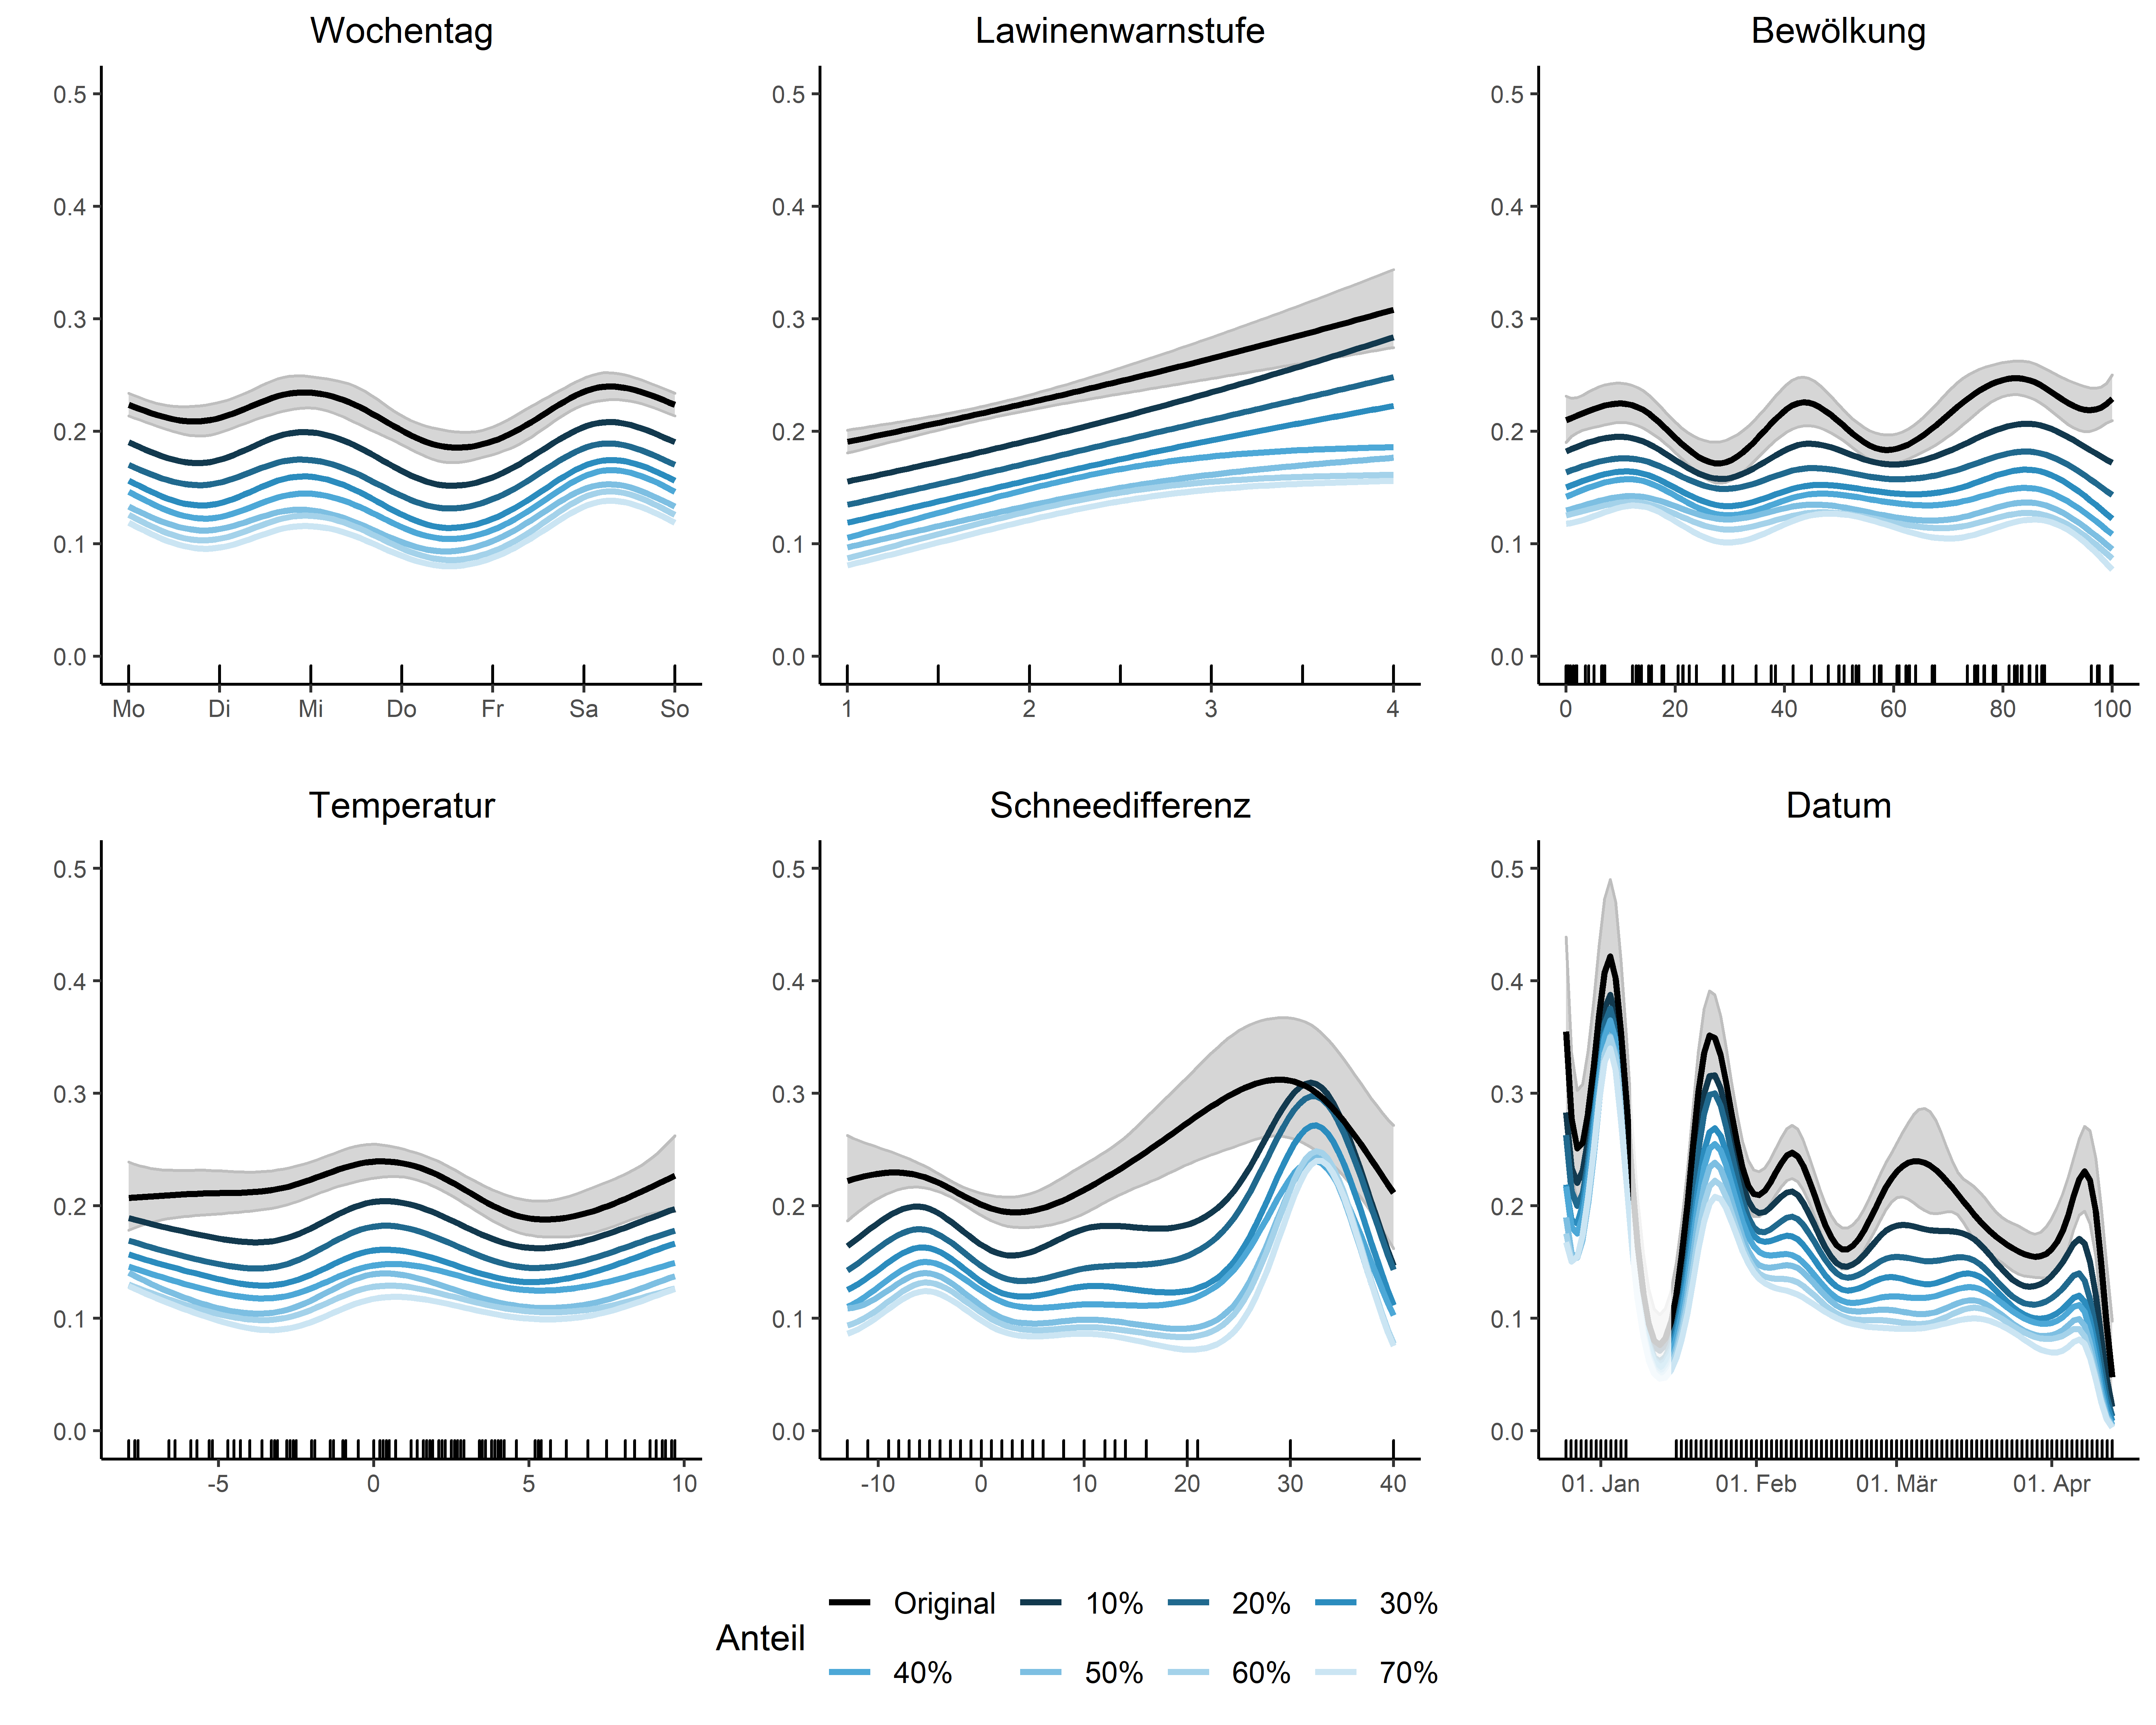
\includegraphics[width=\linewidth]{plots/day_model_general_comparison}
	\caption{ Die glatten Funktionen der Variablen Wochentag, Lawinenwarnstufe, durchschnittliche Tages-Bewölkung, Temperatur, Schneedifferenz für das Tagesmodell}
	\label{pic:day_model_general_comparison}	
\end{figure}
\noindent Abbildung (\ref{pic:day_model_general_comparison}) zeigt im Tagesmodell den Zusammenhang zwischen Anteil an LVS-Geräten und allen nonparametrischen Kovariablen im Original und steigenden Werten für den Anteil an Unterschätzung. \\
Die Verläufe des Zusammenhangs zwischen Anteil an LVS-Geräten und den einzelnen Kovariablen sind für alle Anteile an Unterschätzung sehr ähnlich. \\
Eine kleine Auffälligkeit ist ein größeres Abflachen des Anteils an LVS-Geräten bei einer Lawinenwarnstufe ab 3 bei Anteilen an Unterschätzung von 40\% und höher. Unterschiede zum Original verhalten sich bei allen Werten für Unterschätzung wie vorher für eine Unterschätzung von 22\% beschrieben.

\subsection{Szenario 1 im Zeitmodell}
\begin{table}[htbp]
	\centering
	\caption{Add caption}
	\begin{adjustbox}{max width=\textwidth}
	\begin{tabular}{l|ccc|ccc|ccc|ccc|}
		\multicolumn{1}{r}{} & \multicolumn{3}{c}{Original} & \multicolumn{3}{c}{10\%} & \multicolumn{3}{c}{20\%} & \multicolumn{3}{c}{30\%} \\
		& Koeffizient & p-Wert &       & Koeffizient & p-Wert &       & Koeffizient & p-Wert &       & Koeffizient & p-Wert & \multicolumn{1}{c}{} \\
		\cmidrule{2-13}    (Intercept) & 0.203 & <2e-16 & ***   & 0.165 & <2e-16 & ***   & 0.133 & <2e-16 & ***   & 0.107 & <2e-16 & *** \\
		Ferientag & 0.214 & 0.2   &       & 0.167 & 0.7   &       & 0.133 & 0.9   &       & 0.105 & 0.6   &   \\
		s(Datum) &       & <2e-16 & ***   &       & <2e-16 & ***   &       & <2e-16 & ***   &       & <2e-16 & *** \\
		s(Lawinengefahr) &       & <2e-16 & ***   &       & <2e-16 & ***   &       & <2e-16 & ***   &       & <2e-16 & *** \\
		s(Wochentag) &       & <2e-16 & ***   &       & <2e-16 & ***   &       & <2e-16 & ***   &       & <2e-16 & *** \\
		s(Temperatur) &       & <2e-16 & ***   &       & <2e-16 & ***   &       & <2e-16 & ***   &       & <2e-16 & *** \\
		s(Bewölkung) &       & <2e-16 & ***   &       & <2e-16 & ***   &       & <2e-16 & ***   &       & <2e-16 & *** \\
		s(Schneedifferenz) &       & <2e-16 & ***   &       & <2e-16 & ***   &       & <2e-16 & ***   &       & <2e-16 & *** \\
		\cmidrule{2-13}    \multicolumn{1}{r}{} &       &       & \multicolumn{1}{c}{} &       &       & \multicolumn{1}{c}{} &       &       & \multicolumn{1}{c}{} &       &       & \multicolumn{1}{c}{} \\
		\multicolumn{1}{r}{} &       &       & \multicolumn{1}{c}{} &       &       & \multicolumn{1}{c}{} &       &       & \multicolumn{1}{c}{} &       &       & \multicolumn{1}{c}{} \\
		\multicolumn{1}{r}{} & \multicolumn{3}{c}{40\%} & \multicolumn{3}{c}{50\%} & \multicolumn{3}{c}{60\%} & \multicolumn{3}{c}{70\%} \\
		& Koeffizient & p-Wert &       & Koeffizient & p-Wert &       & Koeffizient & p-Wert &       & Koeffizient & p-Wert & \multicolumn{1}{c}{} \\
		\cmidrule{2-13}    (Intercept) & 0.0899 & <2e-16 & ***   & 0.0771 & <2e-16 & ***   & 0.0664 & <2e-16 & ***   & 0.0582 & <2e-16 & *** \\
		Ferientag & 0.0851 & 0.1   &       & 0.0735 & 0.2   &       & 0.0620 & 0.05  & *     & 0.0537 & 0.02  & * \\
		s(Datum) &       & <2e-16 & ***   &       & <2e-16 & ***   &       & <2e-16 & ***   &       & <2e-16 & *** \\
		s(Lawinengefahr) &       & <2e-16 & ***   &       & <2e-16 & ***   &       & <2e-16 & ***   &       & <2e-16 & *** \\
		s(Wochentag) &       & <2e-16 & ***   &       & <2e-16 & ***   &       & <2e-16 & ***   &       & <2e-16 & *** \\
		s(Temperatur) &       & <2e-16 & ***   &       & <2e-16 & ***   &       & <2e-16 & ***   &       & <2e-16 & *** \\
		s(Bewölkung) &       & <2e-16 & ***   &       & <6e-14 & ***   &       & <6e-14 & ***   &       & <6e-14 & *** \\
		s(Schneedifferenz) &       & <2e-16 & ***   &       & <2e-16 & ***   &       & <2e-16 & ***   &       & <2e-16 & *** \\
		\cmidrule{2-13}    \end{tabular}%
	\end{adjustbox}
	\label{tab:Szenario 1 im Zeitmodell}%
\end{table}%

\noindent Analog wie im Tagesmodell sinken die Koeffizienten für Intercept und Ferientag mit wachsender Unterschätzung. Ab einer Unterschätzung von 30\% ist der Anteil an LVS-Geräten an Ferientagen geringer. \\
Wie im Original sind für alle Werte für die Unterschätzung alle Kovariablen bis auf Ferientag signifikant, ab einer Unterschätzung von 60\% ist auch Ferientag signifikant. \\
\begin{figure}[H]
	\centering
	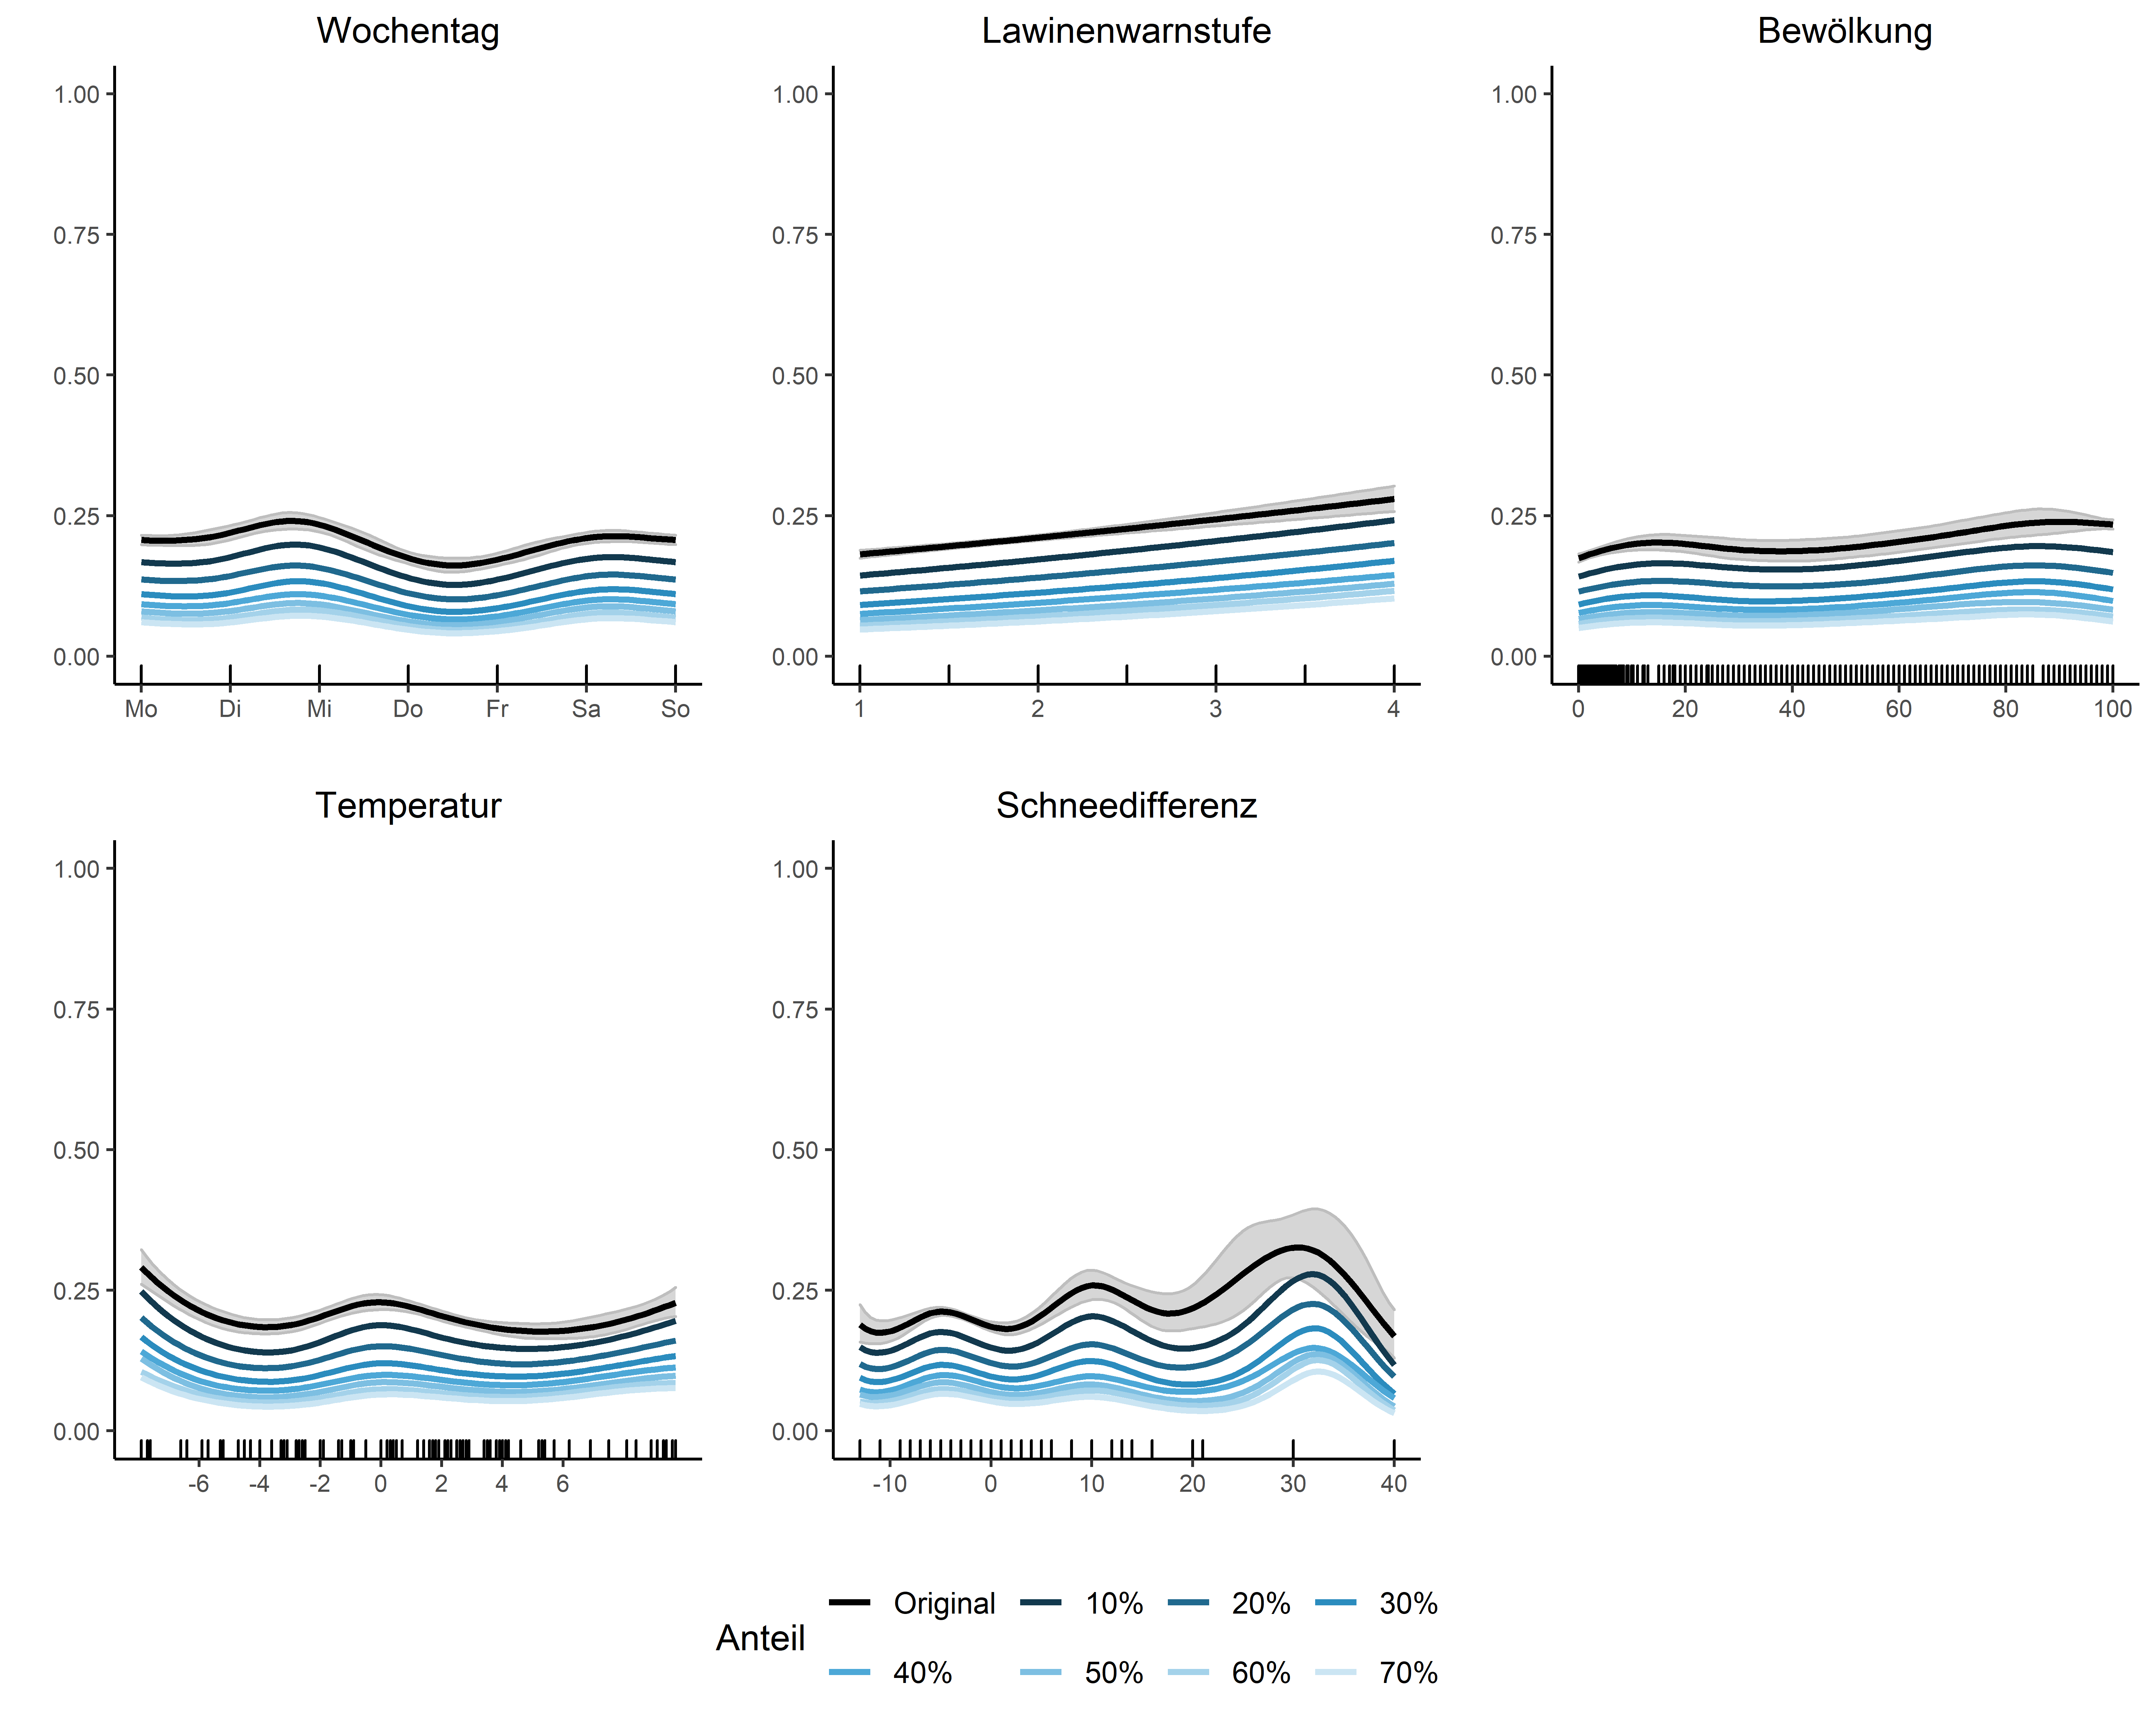
\includegraphics[width=\linewidth]{plots/time_model_general_comparison}
	\caption{ Die glatten Funktionen der Variablen Wochentag, Lawinenwarnstufe, durchschnittliche Tages-Bewölkung, Temperatur, Schneedifferenz für das Zeitmodell}
	\label{pic:time_model_general_comparison}	
\end{figure}
\noindent Abbildung (\ref{pic:time_model_general_comparison}) zeigt im Zeitmodell den Zusammenhang zwischen Anteil an LVS-Geräten und allen nonparametrischen Kovariablen im Original und den verschiedenen Messfehlerszenarien. \\
Wie im Tagesmodell verlaufen die Zusammenhänge zwischen Anteil an LVS-Geräten und den einzelnen Kovariablen für alle Werte an Unterschätzung sehr ähnlich. Größere Unterschiede gibt es weder untereinander noch zum Original.

\chapter{Fazit}
Um die Auswirkungen von Umwelteinflüssen auf die Mitnahme von LVS-Geräten zu untersuchen, wurden zwei Modelle gebildet: einmal wurde dabei nach Datum gruppiert und einmal nach der Uhrzeit. Beim nach Datum gruppierten Modell, dem Tagesmodell, wurden dabei Wochentag, Ferientag, Lawinenwarnstufe, tägliche Durchschnittsbewölkung, Temperatur, Schneedifferenz  und Datum als Kovariablen berücksichtigt. \\
Als signifikant haben sich der Intercept, die Lawinenwarnstufe und das Datum herausgestellt. Bei der Betrachtung des Zeitmodells wurde statt der täglichen Durchschnittsbewölkung die stündliche Bewölkung verwendet und au"serdem Uhrzeit als weitere Variable mit aufgenommen. Hier zeigen sich alle Variablen bis auf Ferientag signifikant. Beide Modelle zeigen eine Abnahme des Anteils von Personen mit LVS-Gerät über die Saison hinweg. Außerdem ist zu erkennen, dass bei höheren Lawinenwarnstufen auch höhere Anteile zu erwarten sind. Das Zeitmodell zeigt, dass Uhrzeit ebenfalls eine Rolle spielt. \\
Eine Analyse der Daten zu den Messfehlern hat ergeben, dass der wahre Wert an vorbeigehenden Kontakten durch den Checkpoint um ca. 22\% unterschätzt wird. Eine besonders hohe Unterschätzung liegt bei einer großen Gruppe an zur selben Minute vorbeigehender Kontakte vor. Ein Vergleich der Modellergebnisse des originalen Datensatzes und verschiedenen Messfehlerszenarien hat ergeben, dass der Verlauf der Zusammenhänge zwischen Anteil an LVS-Geräten und Kovariablen in beiden Modellen für alle Szenarien ziemlich ähnlich ist. Einzig das Szenario mit genereller Unterschätzung zeigt im Tagesmodell mehrere größere Unterschiede, ansonsten kommen diese nur an vereinzelten Stellen vor. \\ Jedoch ändert sich die Höhe des zu erwartenden Anteils je nach Szenario. Auch ein näherer Blick auf das Szenario mit genereller Unterschätzung zeigt bei steigenden Werten für die Unterschätzung nur kleinere Unterschiede zwischen den Szenarien. Auch hier verlaufen die die Zusammenhänge recht ähnlich und unterscheiden sich nur in der zu erwartenden Höhe des Anteils von Personen mit LVS-Gerät. Messfehler, welche den vorgestellten Szenarien entsprechen, ändern somit zwar den Anteil an Personen mit LVS-Gerät den man zu erwarten hat, jedoch nicht die Richtung des Zusammenhanges. \\
Dies führt zu dem Ergebnis, dass, auch bei fehlerhaften Messgeräten, über die Saison hinweg weniger Besucher LVS-Geräte bei sich tragen. Bei höheren Lawinenwarnstufen tragen mehr Besucher ein LVS-Gerät bei sich und über die Saison hinweg ändern sich die Zeiten zu denen mehr Besucher LVS-Geräte bei sich tragen nicht.


\chapter{Anhang}
\begin{table}[htbp]
	\centering
	\vspace{-1em}
	\caption{Concurvity (worst case) vor der Transformation für das Zeitmodell}
	\begin{adjustbox}{max width=\textwidth}
		\begin{tabular}{lccccccc}
			& para & f(Uhrzeit,Datum) & f(Wochentag) & f(Lawinenwarnstufe) & f(Temperatur) & f(Bewölkung) & f(Schneehöhe) \\
			\midrule
			\midrule
			para  & 1.0000 & 0.0000 & 0.2593 & 0.0000 & 0.0000 & 0.0000 & 0.0000 \\
			f(Uhrzeit,Datum) & 0.0000 & 1.0000 & 0.1140 & 0.1466 & 0.6494 & 0.1273 & 0.6110 \\
			f(Wochentag) & 0.2613 & 0.1137 & 1.0000 & 0.0729 & 0.3166 & 0.0604 & 0.1341 \\
			f(Lawinenwarnstufe) & 0.0000 & 0.1466 & 0.0732 & 1.0000 & 0.2559 & 0.1662 & 0.3877 \\
			f(Temperatur) & 0.0000 & 0.6494 & 0.3171 & 0.2559 & 1.0000 & 0.1872 & 0.6004 \\
			f(Bewölkung) & 0.0000 & 0.1273 & 0.0606 & 0.1662 & 0.1872 & 1.0000 & 0.2662 \\
			f(Schneehöhe) & 0.0000 & 0.6110  & 0.1359 & 0.3877 & 0.6004 & 0.2662 & 1.0000 \\
			\bottomrule
		\end{tabular}%
		\label{con1}%
	\end{adjustbox}
\end{table}%

\begin{table}[htbp]
	\centering
	\caption{Concurvity (worst case) nach der Transformation für das Zeitmodell}
	\begin{adjustbox}{max width=\textwidth}
		\begin{tabular}{lccccccc}
			& para & f(Uhrzeit,Datum) & f(Wochentag) & f(Lawinenwarnstufe) & f(Temperatur) & f(Bewölkung) & f(Schneedifferenz) \\
			\midrule
			\midrule
			para  & 1.0000 & 0.0000 & 0.2593 & 0.0000 & 0.0000 & 0.0000 & 0.0000 \\
			f(Uhrzeit,Datum) & 0.0000 & 1.0000 & 0.1140 & 0.1466 & 0.6494 & 0.1273 & 0.2108 \\
			f(Wochentag) & 0.2613 & 0.1137 & 1.0000 & 0.0729 & 0.3166 & 0.0604 & 0.2203 \\
			f(Lawinenwarnstufe) & 0.0000 & 0.1466 & 0.0732 & 1.0000 & 0.2559 & 0.1662 & 0.5220 \\
			f(Temperatur) & 0.0000 & 0.6494 & 0.3171 & 0.2559 & 1.0000 & 0.1872 & 0.3856 \\
			f(Bewölkung) & 0.0000 & 0.1273 & 0.0606 & 0.1662 & 0.1872 & 1.0000 & 0.1434 \\
			f(Schneedifferenz) & 0.0000 & 0.2108 & 0.2201 & 0.5220 & 0.3856 & 0.1434 & 1.0000 \\
			\bottomrule
		\end{tabular}%
		\label{con2}%
	\end{adjustbox}
\end{table}%

\bibliographystyle{chicago}
\bibliography{Report}	

\end{document}